\documentclass[11pt,a4paper,twoside]{report}

% To compile:
% latex report
% bibtex report
% latex report
% latex report

\usepackage[layout,copyright,USenglish,hyperrefurl,twosideshift]{resources/research18}
\usepackage{emptypage} % removes header/footer from empty pages
\usetikzlibrary{fit} % used for the example tikzpicture
\usepackage{pdfpages} % to include external pdf-documents
\usepackage{subcaption}
\usepackage{graphicx}

%\renewcommand{\baselinestretch}{1.2}


%%%%%%%%%%%%%%%%%%%%%%%%%%%%%%%%%%%%%%%%%%%%%%%%%%%%%%%%%%%%%%%%%%%%%%%%%%%%%%%
%%%%% Here the document starts
%%%%%%%%%%%%%%%%%%%%%%%%%%%%%%%%%%%%%%%%%%%%%%%%%%%%%%%%%%%%%%%%%%%%%%%%%%%%%%%
\begin{document}

\pagenumbering{roman}
\pagestyle{plain}
\lfoot{}
\cfoot{\thepage}
\rfoot{}
     
% Title page
\begin{titlepage}
  \begin{center}
    
\includegraphics[height=15mm]{resources/ethlogo} 
    \hfill
    
\includegraphics[height=15mm]{resources/isilogo_plain_bw}

    \rule{\textwidth}{0.5pt}\\[1ex]
    {\Large Fall Semester 2022 \hfill 
      Prof.~H.-A.~Loeliger
      % Prof.~Dr.~A.~Lapidoth
    }

    \vspace{\stretch{5}}
    \LARGE
    Master's Thesis
    % Semester Project

    \vspace{\stretch{8}}
    \Huge\textbf{
        Generative Adversarial Networks for the\\
        Generation of Microphone Array Data
    }

    
    \vspace{\stretch{10}}
    \LARGE{
      Gaspard Ulysse Fragnière
    }
    
    \vspace{\stretch{10}}
  \end{center}
  \rule{\textwidth}{0.5pt}\\[2ex]
  \noindent
  \begin{tabular}{@{}ll@{}}
    \Large Advisor: & \Large Adam Kujawski\\[1ex]
    %\Large Co-Advisor: & \Large Ronald Weasley
  \end{tabular}
\end{titlepage}


\cleardoublepage

% English abstract
\thispagestyle{empty}
\chapter*{Abstract}

This thesis investigates whether Generative Adversarial Network can be used to generate realistic Cross Spectral Matrix (CSM) through their eigendecomposition. Models to generate the eigenvalues' spectrum as well the strongest eigenvector are proposed. The GAN model used to generate those quantities is a Wasserstein GAN with penalized norm of gradient of the critic with respect to its input (WGAN-GP). The method shows that WGAN-GP are suited to generate the eigenvalues spectrum and the strongest eigenvector. Based on those models, a data augmentation scheme allowing to improve the realness of synthetic CSM is introduced. Moreover, this work shows that only a few measured source cases are needed in order to generate data with properties similar to experimental data. Based on the findings of this work, GAN  could be a promising tool to achieve better generalization of deep learning models for source characterization.

\clearpage

\cleardoublepage

% Setup the fancy headers
\pagestyle{fancy}
\renewcommand{\chaptermark}[1]{\markboth{#1}{}}
\renewcommand{\sectionmark}[1]{\markright{\thesection\ #1}}
\fancyhead{}

% Table of contents
\fancyhead[LO]{\scshape \contentsname}
\fancyhead[RO]{\scshape Master's Thesis}
\fancyhead[LE]{\scshape Master's Thesis}
\fancyhead[RE]{\scshape \contentsname}
\pdfbookmark{\contentsname}{contentsbookmarkname}
\tableofcontents

\cleardoublepage

\setcounter{chapter}{0}
\setcounter{figure}{0}
\pagenumbering{arabic}
\fancyhead[LO]{\rightmark}
\fancyhead[RO]{\scshape \chaptername\ \thechapter}
\fancyhead[LE]{\scshape \chaptername\ \thechapter}
\fancyhead[RE]{\textsc{\leftmark}}


%%%%%%%%%%%%%%%%%%%%%%%%%%%%%%%%%%%%%%%%%%%%%%%%%%%%%%%%%%%%%%%%%%%%%%%%%%%%%%%
%%%%% Chapters
%%%%%%%%%%%%%%%%%%%%%%%%%%%%%%%%%%%%%%%%%%%%%%%%%%%%%%%%%%%%%%%%%%%%%%%%%%%%%%%
\chapter{Introduction}


The problem of Acoustical Source Characterization (ASC) is an important problem  of Acoustics. It arises for instance industrial applications such as the characterization of noise on an airplane in a wind tunnel or sound source localization in smart assistants, such as Google Home or Alexa. Traditionaly this problem is tackled with methods based on the physics of sound propagation (e.g. TDoA, beamforming in \cite{merino2019review}) or with statistical inference (e.g. Sparse Bayesian Learning in \cite{gerstoft2016multisnapshot}). Source characterization relies on microphone array data, since accurate result cannot be obtained using data from a single microphone. 

The recent success of Deep Learning (DL) based method in other field of research (e.g. \cite{ronneberger2015u} in Computer Vision) led to believe that Deep Neural Networks (DNN) based approaches could provide state-of-the-art result in solving the ASC problem. State-of-the-art DL-based methods for Source Characterization can be found in \cite{grumiaux2022survey}.

A common issue faced while implementing DL-based methods is that significant quantities of well-structured data are required. In the literature, the data has been obtained using the following approaches:

\begin{itemize}
    \item \textbf{Real Mesurement}: To create the different samples of such a dataset, sounds emitted with a loudspeaker or human voices are recorded in a real acoustic environment. Even though such a method allows for the creation of perfectly realistic samples, it does not come without any issue. Indeed, it is very tedious and time-consuming to record in different environments. Additionally, all the environment for measurement need to physically exists, which limits the quantity of possible samples. Moreover, to build a high quality data set, expensive equipment is required to have an accurate groundtruth (i.e. precisely identify the location of the sources). In the literature, \cite{he2018deep} and \cite{ferguson2018sound} have used such an approach.
    \item \textbf{Synthetic Data}: The sounds used are artificial (i.e. white noise, sine wave). The room acoustic is also simulated. The dry sound is convolved with a simulated Room Impulse Response (RIR) to mimic the effect of room acoustics (e.g. reverberation). Compared to real measurement, this approach allows sample in more diverse environment. Indeed, RIR for rooms of arbitrary size, different source position as well as different dry signals can be used for the training. The issue with such a method is the important amount of time and storage required for the creation of the datasets. E.g. \cite{chakrabarty2017broadband}, \cite{perotin2018crnn} and \cite{adavanne2018direction} created their datasets in this way.
    \item \textbf{Semi-synthetic data}: The creation of such a dataset is similar the creation of synthetic dataset. The difference lies in the fact that the dry sound source used and the RIR are measured and not simulated. Then, the samples of such a dataset are generated by convolving dry sounds with measured RIR. This method is not the best suited, since it is very time-consuming to generate a data set with enough samples for training a DL-based algorithm. Indeed, measuring all the RIR lead to the issues faced with real measurement. \cite{takeda2016sound} use such an approach for to obtain their data.
\end{itemize}

It is to be noted that with the above-mentioned data creation method arises two issues. On one hand, data cannot be created online. Indeed, when using measurement data or semi-synthetic data, measurement need to be performed and stored before any training can occur. On the other hand, synthetic data can be created on the fly when training a model, but this come with the tradeoff that the current synthetization process do not allow to have data as realistic as measurement data.

\section{State of the Art}

In the past years, DL-based approaches have shown to be able to learn and realistically generate complex data structures (e.g. \cite{karras2017progressive} for generation of pictures of faces in the field of Computer Vision). Those breakthroughs lead to believe that similar data generation methods could be used to fix the above-mentioned issues and allow for realistic online data generation. It is therefore needed to identify what acoustic quantities:
\begin{itemize}
    \item have already been generated using a DL approach
    \item are potential feature for a Source Characterization Algorithm.
\end{itemize}

\subsection{Generation of Signal}

\cite{neekhara2019expediting}, \cite{NEURIPS2019_6804c9bc}, \cite{engel2019gansynth} use Generative Adversial Network (GAN) to generate realistic audio waveform. \cite{neekhara2019expediting} and \cite{NEURIPS2019_6804c9bc} specifically focus on the generation of audio waveform conditioned on a spectogram (cGAN). On the other hand, \cite{engel2019gansynth} designed a GAN to generate realistic audio waveform of single music notes played by an instrument. Those approaches focus on generating single channel data and hence might not be fit to generate microphones array data, where each data of the different channels are correlated. It is relevant to note that the GAN designed by \cite{neekhara2019expediting} is the one implemented in \cite{vargas2021improved} in order to compare the accuracy of a network for single source DoA estimation when trained with different sound classes.

\subsection{Generation of Impulse Response}

\cite{papayiannis2019data} introduces a GAN approach to generate artificial Acoustical Impulse Response (AIR) of different environment in order to generate data for a NN used for classification of acoustic environment.

\cite{ratnarajah2021fast} proposes a fast method (NN-based) for generating Room Impulse Response (RIR). The input parameters of the networks used for creating the IR are the desired dimensions of the rectangular room, listener position, speaker position and reverberation time ($T_{60}$).

Currently, these methods only allow to generate impulse responses for only a single listener, hence they would need to be extended to generate several correlated IR per microphone of the array.

\subsection{Generation of potential NN feature}

\cite{bianco2020semi} proposes an approach to generate another acoustic feature: the phase of the relative transfer function (RTF) between two microphones. In this paper a Variational Auto Encoder (VAE) is designed to simultaneously generate phases of RTF and classifying them by their Direction of Arrival (DoA).

\cite{gerstoft2020parametric} use a GAN to generate Sample Cross Spectra Matrices (CSM) for a given DoA. In their approach, the GAN is trained with data only coming from one DoA, making it unable to generate sample for different DoA.

\subsection{Other possible approaches to generate the data}

In \cite{hubner2021efficient} introduce a low complexity model-based method for generating samples of microphones phases. This method proposed is not based on DL. Indeed, it is based on a statistical noise model, a deterministic direct-path model for the point source, and a statistical model. The claim of this paper is that the low complexity of the proposed  model makes it suited for online training data generation. 

\cite{vera2021acoustic} introduce a CNN for denoising (i.e. removing the effects of reverberation and multipath effects) on the Generalization Cross Correlation (GCC) matrix of an array of microphone. More specifically than a CNN, the network used has an encoder-decoder structure.

\section{Aim of the thesis}

Several methods were introduced to generate acoustical quantities, but most do not propose methods that are really suited for multichannel data generation using deep learning. Indeed, only a few papers proposes methods for multichannel data generation. 

Moreover, it is relevant to note that the data used for source characterization in \cite{castellini2021neural}, \cite{lee2021deep}, \cite{ma2019phased}, \cite{xu2021deep} is the Cross Spectral Matrix (CSM), i.e. a direct representation of the signals received in the array of microphone. Those approaches do not use direct recording of microphone input but instead this feature extracted from the raw data. This is crucial because it means that recording, simulating or generating raw microphone data is not necessary, if realistic CSM could be generated directly. 

Therefore, the goal of this thesis is to investigate more general representation of the microphone array data by generating the CSM directly or indirectly, as realistically as possible. It is to be noted that the approach proposed in \cite{gerstoft2020parametric} can be a starting point for the purpose of this thesis. Indeed, this paper introduced a bootstrapping procedure, for the creation of CSM snapshots for a single source position.

\chapter{Fundamentals}

\section{Propagation model and the Cross Spectral Matrix}

If $M$ spatially distributed receivers, $J$ uncorrelated sources and a linear propagation model are considered, then the complex sound pressure at the $m$th microphone is given by

\begin{equation}
    p(\mathbf{r}_m, \omega) = \sum_{j = 1}^{J} h_{mj}(\omega)q(\mathbf{r}_j, \omega) + n(\mathbf{r}_m, \omega)
\end{equation}

Where $\omega$ is the angular frequency and $h_{mj}$ is the transfer function  describing the sound propagation from the $j$th source to the $m$th sensor. $n(\mathbf{r}_m, \omega)$ models independent noise. The above equation can be rewritten as a matrix form

\begin{equation}
    \mathbf{p} = \mathbf{H} \mathbf{q} + \mathbf{n}
\end{equation}

The Cross Spectral Matrix (CSM) or the Sample Covariance Matrix (SCM) is a quantity used in most beamforming algorithm. It can be approximated using Welch's method (see \cite{welch1967use}) as

%Welch's method applies FFT blockwise on the array time data, calculates the CSM for each time data block and finally averages the results.

\begin{equation}
    \label{csm}
    \hat{\mathbf{C}} = \frac{1}{B} \sum_{b = 1}^{B} \mathbf{p}\mathbf{p}^H
\end{equation}

with $B$ snapshots. The CSM is used as the starting point in many microphone array methods, because most information about the location of a source signal are contained in it.

It is to be noted that the CSM can be calculated analytically, or an estimate of the true CSM can be calculated (see \cite{kujawski2022fast}). The latter is often done by from the measured time means of Welch's method (Equation \ref{csm}). Calculating the CSM analytically is fast, but do not yield fully realistic CSM. A third approach is to draw from a Wishart's distribution. This distribution approximates the CSM estimate given by Welch's method without the need to sample the time data. Instead, on can directly sample the elements of the estimated CSM from specific random distributions with:

\begin{equation}
    \hat{\mathbf{C}}_{\mathcal{W}} \sim \frac{1}{B}\mathcal{W}(B)
\end{equation}

with $\mathcal{W}$ the complex Wishart's distribution and $B$ the number of degree of freedom.

\section{Eigendecomposition and Rank I Cross spectral matrix}

A Cross spectral matrix $\mathbf{A}$ of dimension $M \times M$ can be factorized into a canonical form, i.e. a representation by its eigenvalues and eigenvectors using:

\begin{equation}
    \label{eigendecomposition}
    \hat{\mathbf{C}} = \mathbf{V} \mathbf{\Lambda} \mathbf{V}^H
\end{equation}

where $\mathbf{V} = [\mathbf{v}_1^T, \dots, \mathbf{v}_M^T] \in \mathbb{C}^{M \times M}$, $\mathbf{v}_i$ being the $i$th eigenvector and where $\mathbf{\Lambda} \in \mathbb{R}^{M \times M}$ is a diagonal matrix, where $\mathbf{\Lambda}_{ii}$ is the $i$th eigenvalue, corresponding to the $i$th eigenvector. The eigendecomposition is useful because the eigenvalues provide good insights to separate signal from noise., as well as estimating a source strength. 

\cite{sarradj2010fast} uses the eigendecomposition to introduce the Rank I Cross Spectral Matrix. For an approximated CSM $\hat{\mathbf{C}} = \mathbf{V} \mathbf{\Lambda} \mathbf{V}^H$, the Rank I CSM $\hat{\mathbf{C}}_i$ can be computed with:

\begin{equation}
    \label{rank_I_csm}
    \hat{\mathbf{C}}_i = \mathbf{v}_i \mathbf{\Lambda}_{ii} \mathbf{v}_{i}^{H}
\end{equation}

In the next subsection, it will be shown that the rank I CSM can be used to create a beamforming map for only one eigenvalue, corresponding to one audio source. 

\section{Conventional beamforming}

Beamforming is a technique to characterize sound sources using the different signals of an array of microphones. All the microphones of the array record the sound of the source, all with different time delays, depending on the different microphones position, as well as source's location. Using the data from every microphone, a beamforming map can be created, namely a map where the maximum value is at the position of the sound source.

More formally, the situation introduced above, in the propagation model, is considered, namely $M$ microphones organized as an array but this time only with a single source (i.e. $J = 1$), the sound pressure vector $\mathbf{p} \in \mathbb{C}^M$ at every microphone and the corresponding approximated CSM $\hat{\mathbf{C}} = \frac{1}{B} \sum_{b = 1}^{B} \mathbf{p}\mathbf{p}^H$. A scan grid of $N$ potential position of sound sources can be defined. For the sources, the assumption made is that the propagation model is a monopole source. Each position of the grid has a position vector $\mathbf{\xi}_n$. For each grid point $\mathbf{\xi}_n$, the expected signal that would be recorded by each microphone is computed. Every microphone as a position vector $x_m$, for $m \in [1, \dots, M]$. This allows to introduce the  steering vector $g_{n,m} \in \mathbb{C}^M$, defined as 

\begin{equation}
    g_{n,m} = \frac{\exp(-2 \pi i f \Delta t_{n,m})}{4\pi ||x_m -\xi_n||}
    = \frac{\exp \biggl[ -2 \pi i f \frac{||x_m -\xi_n||}{c} \biggr] }{4\pi ||x_m -\xi_n||}  
\end{equation}


where $f$ is the sound frequency under consideration and $\Delta t_{n,m}$ is the propagation time from source $n$ to microphone $m$. $c = 343$ [m/s] is the speed of sound in air. Other definition of the steering vector for different propagation model can be found in \cite{sarradj2012three}.

Using the steering vectors $g_{n,m}$ for $(n,m) \in [1, \dots, N] \times [1, \dots, M]$ and the approximated CSM $\hat{\mathbf{C}}$, the model sound pressure can be compared with the recorded sound pressure. By finding a match, the source location can be identified. To do so, the source autopower per scan grid point $\xi_n$ is computed:

\begin{equation}
    \label{autopower}
    A(\xi_n) = \frac{1}{2} \frac{\mathbf{g}_{n}^H \hat{\mathbf{C}} \mathbf{g}_{n}}{||\mathbf{g}_{n}||^4}
\end{equation}

This provides a source map. An example of source map can be seen in Fig.~\ref{fig:beamforming_example}. Moreover, \cite{sarradj2010fast} shows that equation \ref{autopower}, can also be used with a Rank I CSM $\hat{\mathbf{C}}_i$, giving

\begin{equation}
    A(\xi_n) = \frac{1}{2} \frac{\mathbf{g}_{n}^H \hat{\mathbf{C}}_i \mathbf{g}_{n}}{||\mathbf{g}_{n}||^4}
\end{equation}

\begin{figure}
    \centering
    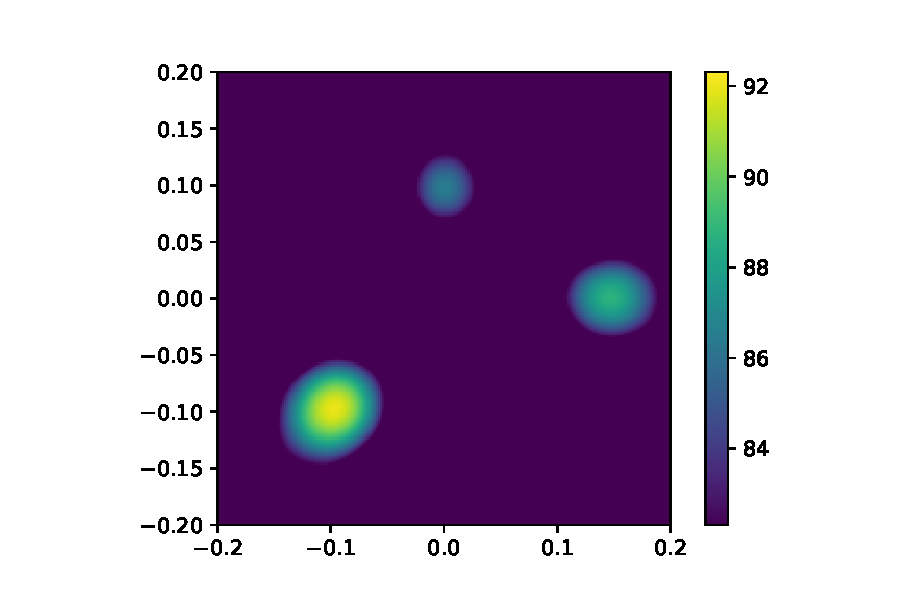
\includegraphics[width=0.7\textwidth]{figs/beamforming_example.pdf}
    \caption{Example of beamforming source map, with three sources.}
    \label{fig:beamforming_example}    
\end{figure}

This gives a beamforming map corresponding to only one single source, the one with associated eigenvalue $\mathbf{\Lambda}_{ii}$.

\section{Helmotz Number}

The Helmotz number $He$ is commonly used in acoustic to represent frequency and is defined as

\begin{equation}
    He = \frac{f \cdot d}{c}  
\end{equation}

where $c = 343$ [m/s] is the speed of sound, $f$ [Hz] the frequency and $d$ [m] the characteristic dimension. It can be noted that the Helmotz is an unitless quantity. 

\section{GAN}

\cite{goodfellow2020generative} introduce a new approach to solve the problem of generative model. The goal is to learn the probability distribution that was used to generate samples, by observing them.

The method introduced in this paper is called Generative Adversial Network (GAN). The idea is to create a game (in the game theory sense) where two networks compete against each other. The first network is called a discriminator and its goal is to determine real from fake samples. The other network is a  generator with the aim to produce data realistic enough that the discriminator cannot determine that it has been generated.

The generator takes as input a random vector and use it generate a sample. This random vector is referred to as latent variable. The vector space of latent variable is called latent space. After training, the generator should be a mapping from the latent space to the data space. The latent space is  a representation of smaller dimension of the data space.

The discriminator takes as input a real or generated sample and predicts its authenticity. The discriminator is a simple binary classifier. The real sample come from the datasets and the fake are outputs of the generator.

Both models are trained simultaneously. First the generator create a batch of fake sample. This batch is then fed to the discriminator, alongside a batch of real samples. For each of them, the discriminator makes a prediction about their authenticity. The discriminator then gets updated based on how accurate it was at classifying samples and the generator based on how many times fake sample were able to fool the discriminator. It can be observed here that the training of both networks is supervised, on the contrary of typical generative models.

In a gaming theory framework, both networks are competing in a zero-sum game. This means that if one network performs well at its task and gets rewarded by little weights update, the other must have performed poorly and hence gets penalized by heavy weights updated. E.g. if the discriminator was successful at classifying all samples, it means that the generator had not been able to fool the discriminator by producing any realistic fake samples.  


%\section{DCGAN}

%\cite{radford2015unsupervised} introduce GAN, but unlike in \cite{goodfellow2020generative}, the architecture of the discriminator and generator is not achieved with regular perceptron, but with Convolutional layer. First, it needs to be reminded how a regular perceptron layer works. For an input vector $\mathbf{x} \in \mathbb{R}^k$ and output vector $\mathbf{y} \in \mathbb{R}^l$, a perceptron layer consists of two parts:

%\begin{itemize}
%    \item an activation $\mathbf{a} = \mathbf{W} \mathbf{x} + \mathbf{b}$
%    \item a non-linearity $y = f(\mathbf{x};\theta) = \sigma(\mathbf{a})$
%\end{itemize}

%where $\mathbf{W} \in \mathbb{R}^{l \times k}$ are the weights of the perceptron and $\mathbf{b} \in \mathbb{R}^l$ its bias. $\sigma(\cdot)$ is called the activation function and is the source of non linearity in neural networks. An example of such activation function is the Rectified Linear Unit (ReLU) where:

%\begin{equation}
%    \sigma_{\text{ReLU}}(\mathbf{a}) = [\max(a_0, 0), \dots, \max(a_{l-1}, 0)]^T
%\end{equation}

%The architecture of a convolutional layer can now be introduced. Without loss of generality, the assumption that the network receives as input an square image with a single channel is made, i.e. $\mathbf{H_0} \in \mathbb{R}^{d_0 \times (m \times m)}$ with $d_0 = 1$, transforms it with one square kernel, i.e. $\mathbf{K} \in \mathbb{R}^{s \times (r \times r)}$ with $s = 1$ to output another square image with a single channel, i.e. $\mathbf{H_1} \in \mathbb{R}^{d_1 \times (n \times n)}$, with $d_1 = 1$

%The relationship between input image $\mathbf{H_0} \in \mathbb{R}^{m \times m}$, output image $\mathbf{H_1} \in \mathbb{R}^{n \times n}$ and kernel $\mathbf{K} \in \mathbb{R}^{r \times r}$ is defined as:


%\begin{itemize} 
%    \item an activation $\mathbf{A} = \mathbf{H_0} \ast \mathbf{K}$
%    \item a non-linearity $\mathbf{H_1}_{(i,j)} = \sigma(\mathbf{A}_{(i,j)})$ 
%\end{itemize}

%\cite{radford2015unsupervised} proposes a set of constraint that makes the use of convulotional layers possible in GAN setting.


\section{WGAN}

\cite{arjovsky2017wasserstein} introduce a new type of Generative Adversial Network (GAN): the Wasserstein GAN (WGAN). The claim is that WGAN improves the stability in learning and get rid of typical problem of the traditional GAN approach such as Mode Collapse or Convergence failure. Mode collapse is when a GAN fails to fully converged because the generator learns only to generate a subset of the real data in order to fool the discriminator. This leads to a situation where the GAN is able to produce realistic data but not all kind of data, which is not a desired behavior. More specifically, \cite{arjovsky2017wasserstein} provides the following insights:

\begin{itemize}
    \item Introduces the Earth-Mover (EM) or Wasserstein distance. It is a metric used to quantify the distance between two probability distributions.
    \item Analyses how the EM distance behaves compared to other distances between probability distribution (e.g. Kullback-Leibler distance).
    \item Defines a GAN minimizing an approximation of the EM distance, namely the WGAN.
    \item Shows that, unlike traditional GANs, WGANs do not need to maintain a balance when training the discriminator and generator. Indeed, in regular GAN approach, it was crucial to avoid the discriminator to become too good before the generator, since this would prevent the generator to learn any distribution.
    \item Provides useful insights to determine whether the WGAN has converged or not. Determining convergence was a hard problem with the regular GAN approached and it was typically assessed by visually determining if the produced samples were realistic or not.
\end{itemize}


\subsection{The Earth-Mover or Wasserstein distance}


The goal of WGAN, remains the same as GAN, namely solving the problem of generative model. More precisely, this mean approximating the probability distribution $P_r$ of some data by a distribution $P_{\theta}$. For this reason, it is necessary to have metrics to quantify distance between two probability distributions $P_r$ and $P_m$. Example of such distances are the Kullback-Leibler divergence or the Jensen-Shannon divergence. In WGAN, the distance used is the Earth-Mover (EM) distance or Wasserstein-1, defined as 

\begin{equation}
    W(\mathbb{P}_r, \mathbb{P}_m) = \inf_{\gamma \in \Pi(\mathbb{P}_r, \mathbb{P}_m)} \mathbb{E}_{(x,y) \sim \gamma} [||x-y||]
\end{equation}

Where $\Pi(\mathbb{P}_r, \mathbb{P}_m)$ is the set of all joint distribution $\gamma(x,y)$ whose marginals are respectively $\mathbb{P}_r$ and $\mathbb{P}_m$. Informally, $\gamma(x,y)$ shows how much "mass" must be carried to transform $\mathbb{P}_r$ into $\mathbb{P}_m$. The EM distance is then "the cost" of the optimal "transport".

\cite{arjovsky2017wasserstein} shows that the EM distance is better than the following metrics to quantify distances between probability distributions, namely

\begin{itemize}
    \item the Total Variation metric, defined as
    \begin{equation}
        \delta(P_r, P_g) = \sup_{A} |P_r(A) -  P_g(A)|
    \end{equation}
    \item The Kullback-Leibler divergence defined as
    \begin{equation}
        KL(P_r||P_g) = \int_x  \log \Bigl( \frac{P_r(x)}{P_g(x)} \Bigr) P_r(x) dx
    \end{equation}
    It is important to note that $KL(P_r||P_g) \neq KL(P_g||P_r)$ (i.e. not symmetric)
    \item The Jensen-Shannon divergence. For $P_m$ a mixture distribution with $P_m = \frac{P_r + P_g}{2}$, the Jensen-Shannon divergence is defined as  
    \begin{equation}
        JS(P_r, P_g) = \frac{1}{2} KL(P_r||P_m) + \frac{1}{2} KL(P_g||P_m)
    \end{equation}
\end{itemize}

\cite{arjovsky2017wasserstein} uses the following example to explain the relevance of the EM distance. The data distribution $(0, y)$ with, $y \sim U[0,1]$ and the family of distribution $P_{\theta}$, where $P_{\theta} = (\theta, y)$ again with $y \sim U[0,1]$ are considered. The distance metric should move closer to zero, as $\theta \rightarrow 0$. For such a distribution, this is how the different distances behave:

\begin{itemize}
    \item Total Variation
    \begin{equation}
        \delta(P_0, P_{\theta}) = 
        \begin{cases}
            1 & \text{if } \theta \neq 0\\
            0 & \text{if } \theta = 0
        \end{cases}
    \end{equation}
    \item Kullback-Leibler Divergence
    \begin{equation}
        KL(P_0 || P_{\theta}) = KL(P_{\theta} || P_0) =
        \begin{cases}
            +\infty & \text{if } \theta \neq 0\\
            0 & \text{if } \theta = 0
        \end{cases}
    \end{equation}
    \item Jensen-Shannon Divergence  
    \begin{equation}
        JS(P_0, P_{\theta}) = 
        \begin{cases}
            \log(2) & \text{if } \theta \neq 0\\
            0 & \text{if } \theta = 0
        \end{cases}
    \end{equation}
    \item the Earth mover distance
    \begin{equation}
        W(P_0, P_{\theta}) = |\theta|
    \end{equation}
\end{itemize}

This simple example shows that there exist distributions for which the Total Variation, the Kullback-Leibler Divergence and the Jensen-Shannon Divergence do not converge, whereas the Earth mover Distance does. \cite{arjovsky2017wasserstein} then confirms the insight provided by this example with the two following theorems (without proof here, but the proofs can be found in \cite{arjovsky2017wasserstein})

\textbf{Theorem 1:} Let $P_r$ be a fixed distribution. Let $Z$ be a random variable. Let $g_{\theta}$ be a deterministic function parametrized by $\theta$ and let $P_{\theta} = g_{\theta}(Z)$. Then

\begin{enumerate}
    \item If $g$ is continuous in $\theta$, then so is $W(P_r, P_{\theta})$
    \item If $g$ is sufficiently nice, then $W(P_r, P_{\theta})$ is continuous everywhere and differentiable almost everywhere.
    \item Statements 1 and 2 do not hold for neither $JS(P_r, P_{\theta})$, $KL(P_r||P_{\theta})$ or $KL(P_{\theta}||P_r)$.
\end{enumerate}

This first theorem shows that out of the four loss functions above-mentioned, only the Earth-Mover has some guarantees of both continuity and differentiability, which are nice guarantees for a loss function.

\textbf{Theorem 2:} Let $P$ be a distribution and $(P_n)_{n \in \mathbb{N}}$ be a sequence of distributions. The following is true

\begin{enumerate}
    \item The following statements are equivalent:
    \begin{itemize}
        \item $\delta(P_n, P) \rightarrow 0$
        \item $JS(P_n, P) \rightarrow 0$
    \end{itemize}
    \item The following statements are equivalent:
    \begin{itemize}
        \item $W(P_n, P) \rightarrow 0$
        \item $P_n \rightarrow P$, with here "$\rightarrow$" being convergence in distribution for random variables. 
    \end{itemize}
    \item $KL(P_n||P) \rightarrow 0$ or $KL(P||P_n) \rightarrow 0$ implying statement 1.
    \item Statement 1 implies statement 2.
\end{enumerate}

The above theorem proves that every distribution that converges under the Kullback-Leibler divergence (in any direction), the Jensen-Shannon divergence or the Total Variation also converges under the Earth-Mover distance. It also shows that a smaller difference between two probability distribution implies a smaller EM distance. 

Unfortunately the EM distance is intractable, due to the infimum part in its equation. But using the Kantorovich-Rubinstein duality, it can be reformulated as:



\begin{equation}
    W(\mathbb{P}_r, \mathbb{P}_{\theta}) = \sup_{||f||_L \leq 1} \mathbb{E}_{x \sim \mathbb{P}_r} [f(x)] - \mathbb{E}_{x \sim \mathbb{P}_{\theta}} [f(x)] 
\end{equation}

Where the supremum is over 1-Lipschitz functions. It is important to note that if $||f||_L \leq 1$  is replaced by $||f||_L \leq K$, i.e. consider also the K-Lipschitz functions, then $K \cdot W(\mathbb{P}_r, \mathbb{P}_{\theta})$ can be obtained. Hence, for a family of functions $\{f_w\}_{w \in \mathcal{W}}$ (all functions being K-Lipschitz), it boils down to solving the optimization problem:

\begin{equation}
    \max_{w \in \mathcal{W}}  \mathbb{E}_{x \sim \mathbb{P}_r}[f_w(x)] - \mathbb{E}_{z \sim p(z)}[f_w(g_{\theta}(z))]
\end{equation}

Note: the solution of the above-mentioned problem can be approximated with a Neural Network with weights $\mathcal{W}$. $\mathcal{W}$ need to be compact to assure that the function $f_w$ are K-Lipschitz. Therefore, in order to have $\mathcal{W}$ being compact, \cite{arjovsky2017wasserstein} proposes to simply clip the weights, such that they lay in a small box $[-c, c]^l$, e.g. with $c = 0.01$

\subsection{Necessary changes to turn a GAN into a WGAN}

Implementation of a WGAN requires a few changes from implementation of a regular GAN, i.e. 

\begin{itemize}
    \item Use a linear activation function in the output layer of the "discriminator" model (instead of sigmoid). The "discriminator" then becomes a critic that quantify the realness of a sample, instead of discriminating between real or fake.
    \item Use Wasserstein loss to train the critic and generator models that promotes larger difference between scores for real and generated images. 
    \item Constrain critic model weights to a limited range after each mini batch update (e.g. [-0.01,0.01]). As seen above, this is to ensure, that the function estimated in the for approximating the Wasserstein distance are K-lipschitz, a necessary condition.
    \item Update the critic model more times than the generator each iteration (e.g. 5). Contrary as in a GAN, this is not an issue. Indeed, switching to the EM distance, allows for more stability when training the two networks in the WGAN. Moreover, the fact that the EM distance is continuous and differentiable means that the critic should be trained until optimality.
    \item Use the RMSProp version of gradient descent with small learning rate and no momentum (e.g. 0.00005).
    
\end{itemize}


\section{WGAN-GP}

As seen above, WGAN improve the stability in training the critic ($\approx$ discriminator). But it is still subject to poor sample generation, convergence failure or mode collapse. This is due to the weight clipping happening while training the critic. In order to remedy to this, \cite{DBLP:journals/corr/GulrajaniAADC17} propose to replace weight clipping by the introduction of a penalization of the norm of gradient of the critic with respect to its input. The issue is that trying to orient the critic to 1-Lipschitz function by weight clipping, biases the critic for too simple function. \cite{DBLP:journals/corr/GulrajaniAADC17} observes that implementing the Lipschitz constraint using weights clipping leads to either exploding or vanishing gradient, unless the threshold $c$ used for the clipping is carefully fine-tuned.

\subsection{The gradient penalty}

In order to enforce the Lipschitz constraint, \cite{DBLP:journals/corr/GulrajaniAADC17} proposes to add a penalty term to the loss function. The loss function then becomes: 

\begin{equation}
    L = L' + P
\end{equation}

where:

\begin{itemize}
    \item Original loss function: 
    \begin{equation}
        L' = \mathbb{E}_{\mathbf{\tilde{x}} \sim \mathbb{P}_g} [D(\mathbf{\tilde{x}})] - \mathbb{E}_{\mathbf{x} \sim \mathbb{P}_r} [D(\mathbf{x})]
    \end{equation}
    \item Penalty:
    \begin{equation}
        P = \lambda \mathbb{E}_{\hat{\mathbf{x}} \sim \mathbb{P}_{\hat{\mathbf{x}}}}[(||\nabla_{\hat{\mathbf{x}}} D(\hat{\mathbf{x}})-1||)^2]
    \end{equation}
\end{itemize}

The goal of the penalty is to enforce the 1-Lipschitz constraint. Indeed, by definition, a function is 1-Lipschitz if and only if its gradient norm is smaller or equal to 1 everywhere. It can be easily seen that the penalty is here to enforce this constraint. In order to make such a penalty tractable, a soft version of the penalty is considered, where the constraint is only enforced on the gradient norm of a few random samples $\hat{\mathbf{x}} \sim \mathbb{P}_{\hat{\mathbf{x}}}$.

The sampling distribution $\mathbb{P}_{\hat{\mathbf{x}}}$ is defined by sampling uniformly on on a line between a pair of points respectively sampled from $\mathbb{P}_{r}$ and $\mathbb{P}_{g}$. This was proven experimentally to give sufficiently good results.

In \cite{DBLP:journals/corr/GulrajaniAADC17}, the penalty coefficient was set always to 10 in all experiences done. No batch normalization was used in \cite{DBLP:journals/corr/GulrajaniAADC17}. They claim that batch normalization shifts the discriminator problem from trying to match a single input to a single output from trying to match a batch input to a batch output. This makes the penalty invalid, since the penalization is performed with each input individually and batch normalization introduce correlation between samples. Instead of batch normalization, \cite{DBLP:journals/corr/GulrajaniAADC17} recommends layer normalizations.

\section{Assessing performances of a WGAN or WGAN-GP compared to GAN} \label{sec:assessing_perf}

A problem with regular GANs (from \cite{goodfellow2020generative}) is that it is really hard to know when a good model has been found, from looking only at the loss function. The quality of a model is typically assessed by visually looking at the generated sample and deciding if they are realistic or not. But \cite{arjovsky2017wasserstein} shows that in a WGAN, the Wasserstein loss is a meaningful loss function, that is correlated with the quality of the sample produced by the generator. This is not true in a regular GAN and is actually one of the main selling point of a WGAN over GAN.

\cite{DBLP:journals/corr/GulrajaniAADC17} shows that this property of the WGAN still holds true for the WGAN-GP. The critic loss should typically start at zero, then drops and work its way back to zero. This is when the WGAN-GP has converged and is hence producing realistic samples.

\chapter{Methods}

In this chapter, the investigated methods of the thesis for the approximation of the CSM are introduced. The idea behind these methods takes its root in \cite{gerstoft2020parametric}. In \cite{gerstoft2020parametric}, A WGAN-GP is used to generate the $B$ snapshots $\mathbf{p} \mathbf{p}^H$ (see equation \ref{csm}). In this thesis, WGAN-GPs are designed to generate the eigenvalues and eigenvectors of the eigendecomposition of a CSM (see equation \ref{eigendecomposition}).

This choice of generating the CSM through its eigendecomposition instead of generating directly the CSM or generating snapshot as in \cite{gerstoft2020parametric} can be justified. On the one hand, the CSM is a complex data structure and building a model to learn its probability distribution is a hard task. Indeed, CSM are complex and hermitian matrices. On the other hand, generating the snapshots is a computationally extensive.

Moreover, generating the eigenvalues comes with two advantages. First, a model to generate eigenvalues of CSM would allow for a quick data augmentation strategy. By using generated eigenvalues and real eigenvectors, the datasets could be extended. This is of particular interest, since the measurement datasets at our disposal is too small for a learning task. Then, being able to generate the eigenvalues could be used to realify synthetic CSM. As it will be shown, one significative difference between synthetic CSM and CSM from real measurement is the steepness in the decay of the eigenvalues spectrum.

Generating the eigenvectors also comes with benefits. All the positional information of a source (and its coherent component) are contained in the eigenvectors. In free-field synthetic source cases, an eigenvector is different to a measured one which holds the source position and the information from coherent reflections of the environment. In this sense, Replacing the strongest eigenvector with a generated one trained from measured data would probably already improve the degree of realism. It is to be noted that the strongest eigenvector contains the information about the source, in the case of a single source.

Moreover, the eigenvectors can be normalized and the eigenvalues scaled such that they all lie in $[0,1]$. Both these normalization and scaling processes could allow to reduce the size of the space of data to generate and hence improve performances.

Each of the above-mentioned techniques are of valuable interest for supervised learning of deep learning models. Moreover, data does not need to be saved on disk and can be created swiftly, once the models are trained. 

Finally, it is worth mentioning that the data generated in this thesis contains only a single source (plus some noise). But this can be extended to  the multiple source cases since it can be created by superposition of individual CSM.

As mentioned in the introduction using only real measurement was not a feasible approach, since there are enough measurement available required for training. For this reason, the chosen approach was to first pretrain the models using the eigendecomposition of synthetic CSM and then fine-tune the model using eigendecomposition of CSM of recorded pressure vectors $\mathbf{p}$. 

Different approaches to generate the CSM from their eigendecomposition have been considered. Those approaches were the following:

\begin{itemize}
    \item Generating the eigenmodes. The eigenmodes are the eigenvectors scaled by their respective eigenvalues. This method is not explored in depth in this thesis, since it was not producing good results. The problem with the eigenmodes is that the amplitude of the least important modes become too small to be modeled accurately. 
    \item Generating only the eigenvalues.
    \item Generating only the levels of eigenvalues.
    \item Generating only a single eigenvector. More specifically only the strongest eigenvector is generated, since it is the one containing the information about the strongest source, which is the only source in our case. 
    \item Generating all the remaining weakest eigenvectors. This approach has not been investigated in depth. Trying to generate the remaining weakest eigenvector the same way as done for the strongest eigenvector has been tried but not successfully.  
\end{itemize}

\section{Data}

For training the networks designed in this thesis, two kinds of data were used, namely synthetic and measurement datasets. In the next subsections, the data available for training the network is explained. 

\subsection{Synthetic Data}

When a specific measurement was chosen to create the measurement dataset, its source's position was used to create the corresponding synthetic data. The synthetic CSM were sampled from the complex Wishart's distribution. The number of degree of freedom was set to $4 \times M = 256$, since they are $M = 64$ microphones. Moreover, some noise was added to the synthetic CSM, such that the SNR of synthetic data was approximately matching the one of the measurement data. Here the SNR was approximately 60dB. 

When creating the CSM from the synthetic data, the CSM corresponding to the Helmotz number $He = 16$ were created. In the case of the synthetic data, the characteristic dimension was $d_s = 1\,$m, hence the frequency related to the Helmotz number $He$ was $f = 5.488\, \mathrm{kHz}$. The source position used in the synthetic was $(x \cdot d_s,y \cdot d_s, z \cdot d_s) = (-0.0614,-0.0757, 0.5)$.

\subsection{Measurement}

In order to generate realistic data, measurement have been performed. Existing microphone array data that stems from a measurement campaign in 2022 was used. An example of the measurement setup is displayed in Fig.~\ref{fig:full_measurement_setup}. It is made of sound sources located at different position $(x \cdot d_m,y \cdot d_m, z \cdot d_m)$ in a $1 \cdot d_m\,$m $\times$ $1 \cdot d_m\,$m plane located $0.5 \cdot d_m\,$m in front an array of 64 microphones. In the case of the measurement data, the characteristic dimension $d_m$ was equal to $1.46\,$m, which is the aperture size $AP$ of the microphone array. Every measurement corresponds to single source case, at a different position for every measurement. All measurements have a duration $10\,$s and a sampling frequency of $51.2\,$kHz. It is to be noted here that the SNR of the recordings was of 62.5dB. For the recordings, the microphones were organized in Vogel's spiral pattern, with the central one acting as the reference microphone. Fig.~\ref{fig:microphone_array} shows the microphone array used in the measurement setup. The measurements are sound pressure $\mathbf{p} \in \mathbb{C}^{64}$ at the 64 microphones of the array.

\begin{figure}
    \centering
    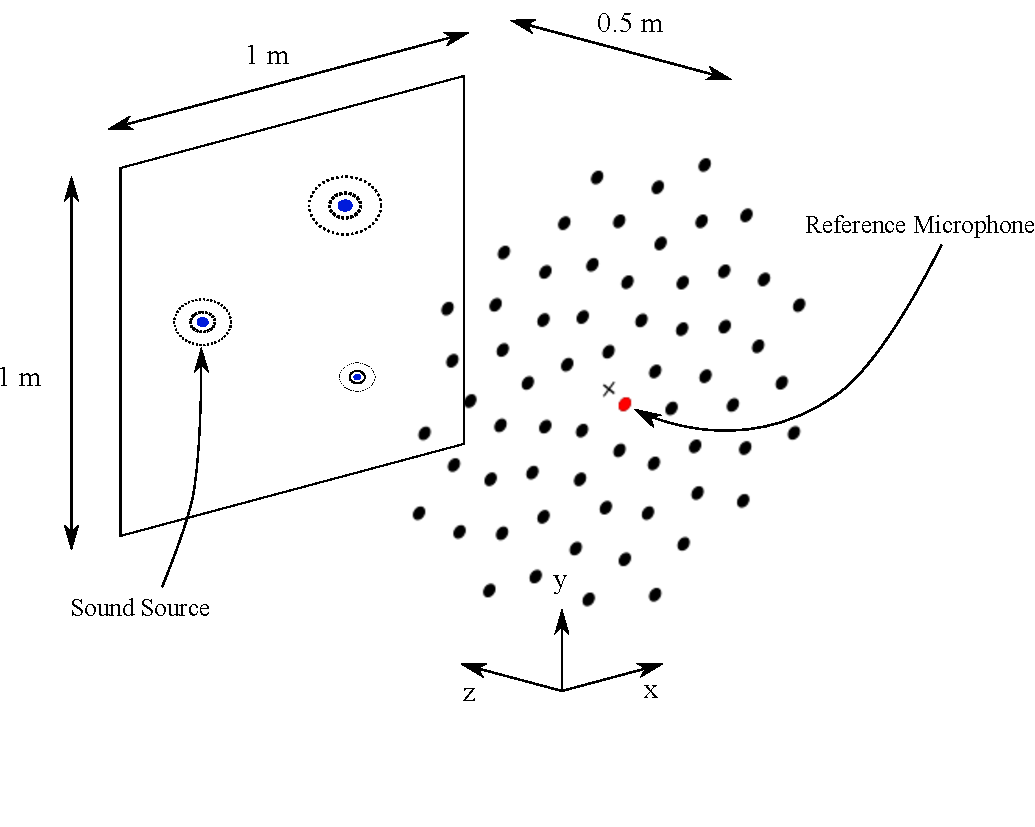
\includegraphics[width=1\textwidth]{figs/full_measurement_setup.pdf}
    \caption{Example of the measurement setup used, with three audio sources. This is image is only for illustration purposes. In the actual performed measurement, there was only one audio source. Moreover, the dimension showed in the picture are for an aperture size of $1\,$m, whereas in the actual performed measurement, the aperture size was of $1.46\,$m. This means that in the actual setup every dimension were actually 1.46 times bigger than in the image. This image is taken from \cite{kujawski2022acoupipe}}
    \label{fig:full_measurement_setup}
\end{figure} 

\begin{figure}
    \centering
    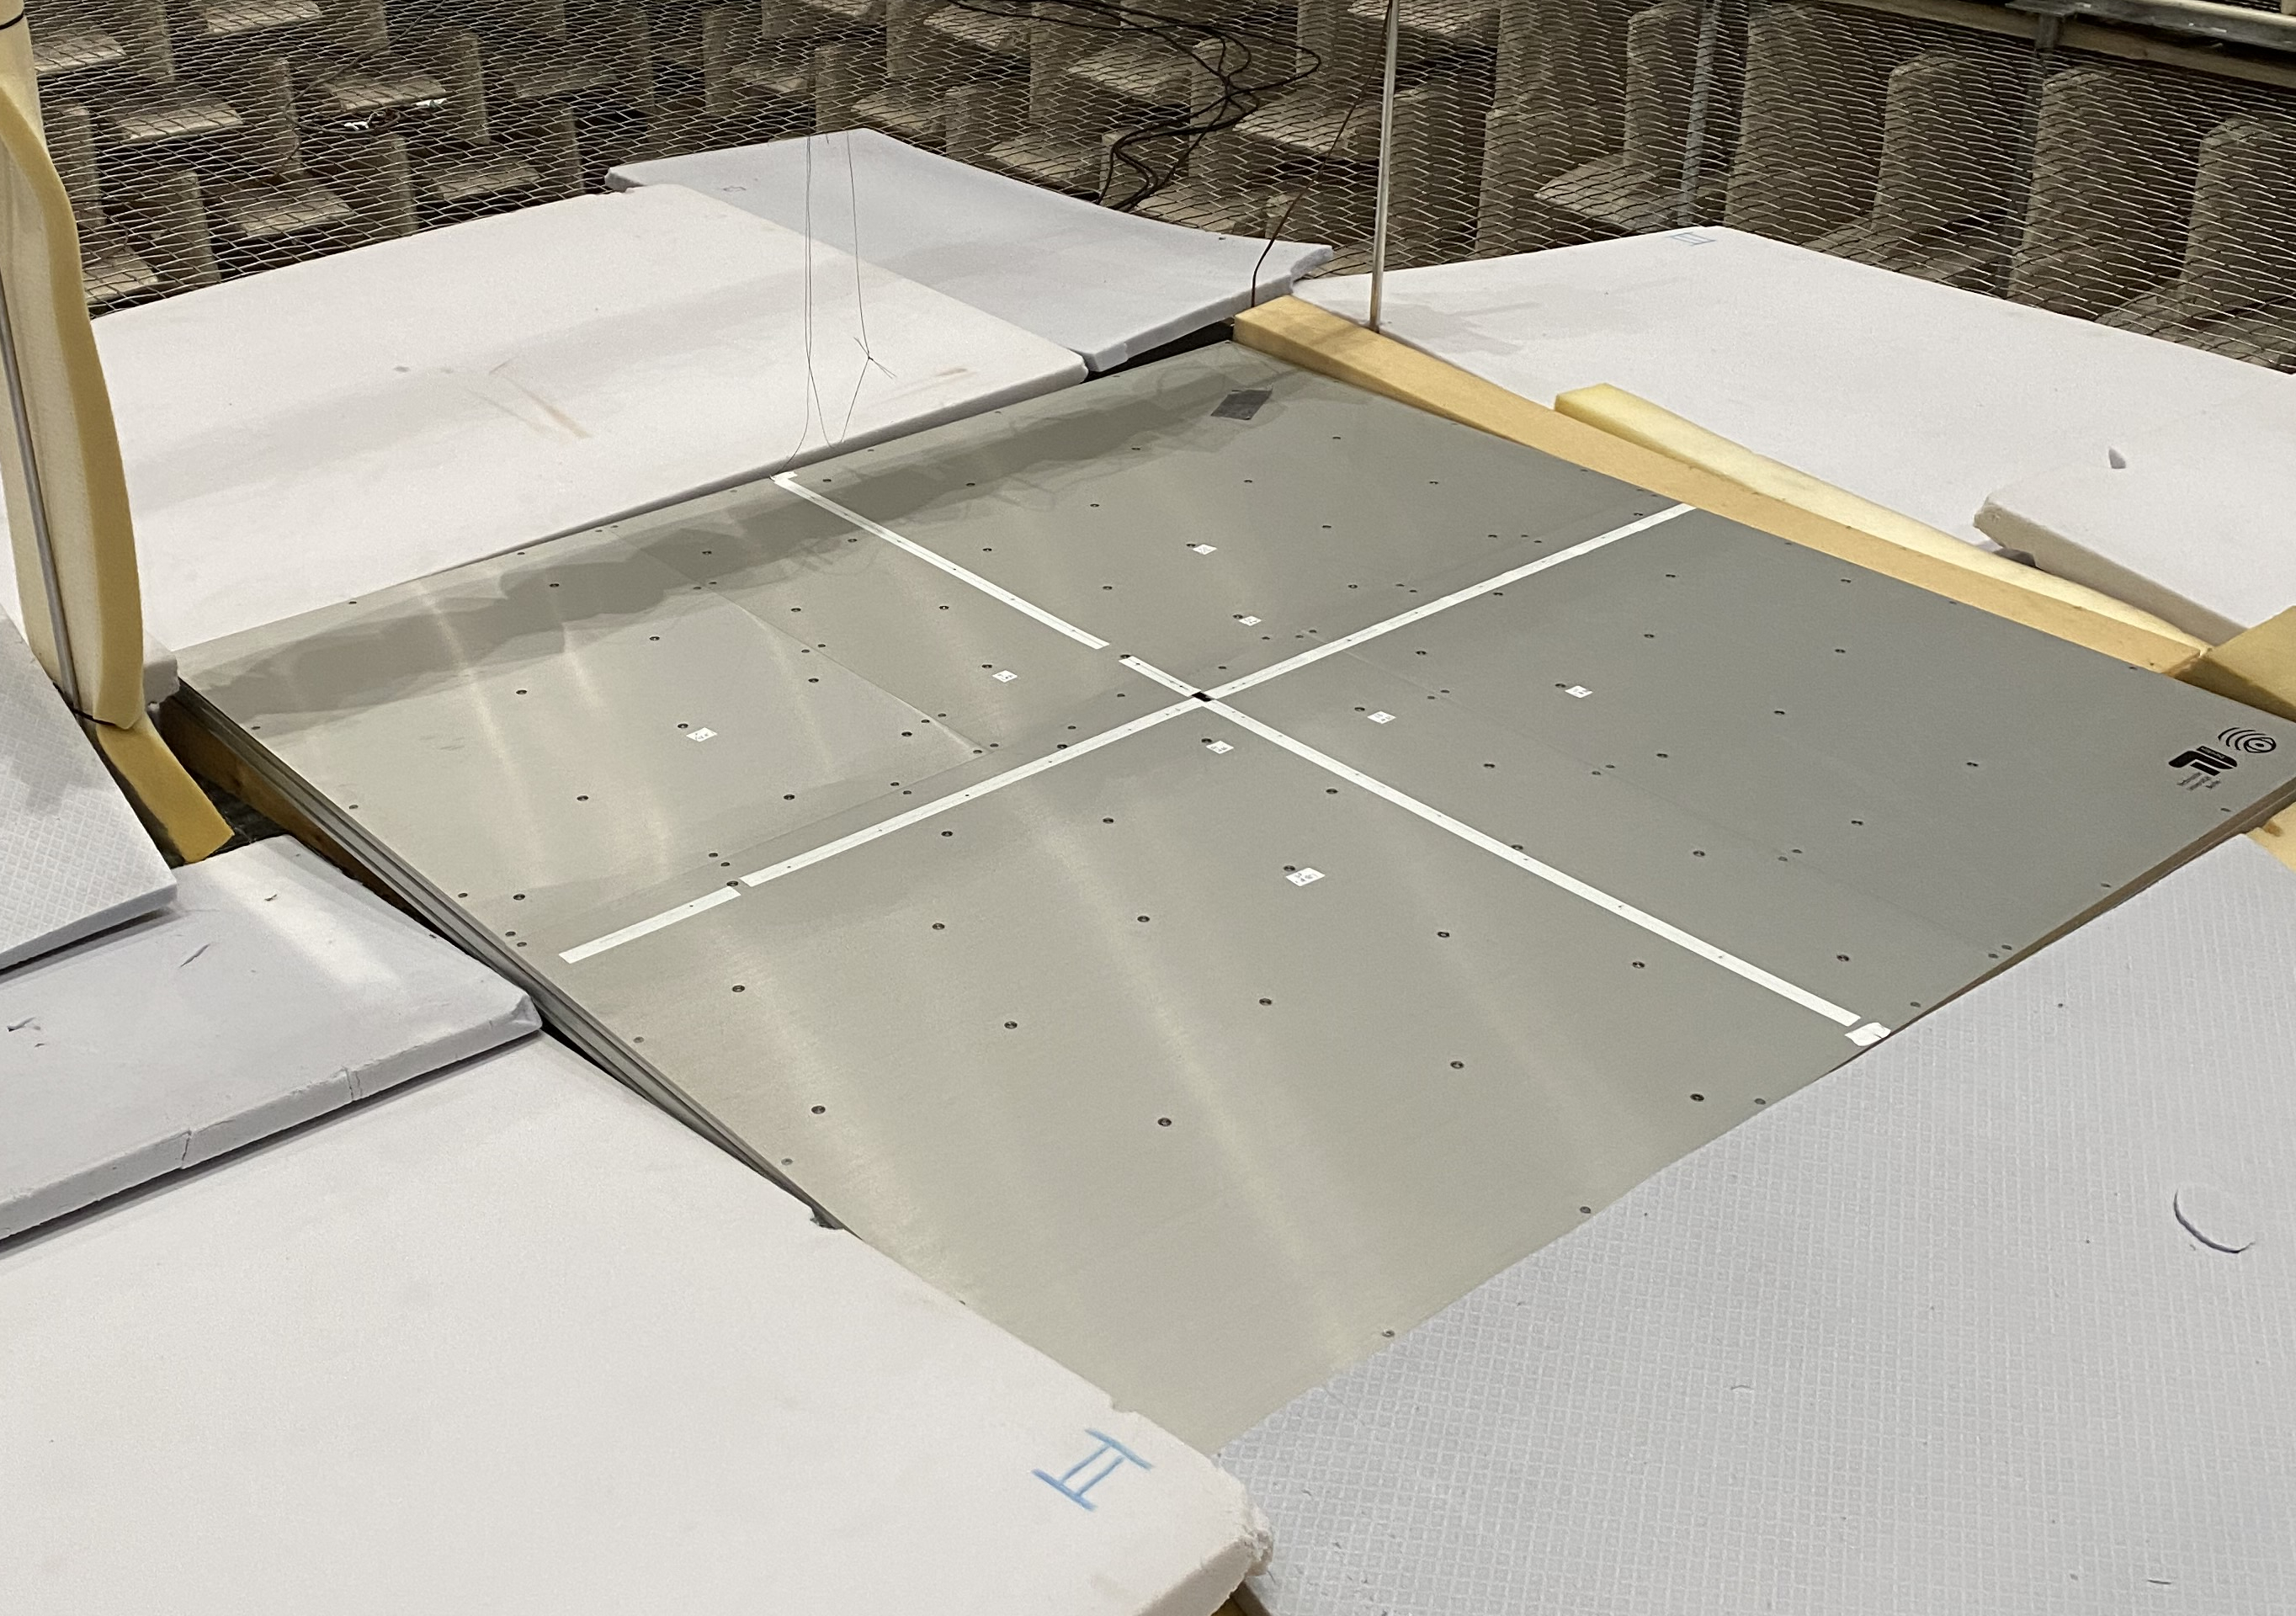
\includegraphics[width=0.8\textwidth]{figs/microphone_array_cropped.jpg}
    \caption{Picture of the array of microphone used to create the measurement.}
    \label{fig:microphone_array}
\end{figure}


From the recorded sound pressure vector $\mathbf{p}$, Welch's method (i.e. equation $\ref{csm}$) is used to compute approximated CSM $\hat{\mathbf{C}}$. From \cite{gerstoft2012eigenvalues}, it is known that the number of snapshots $B$ needed to be at least 4 times the number of receivers $M$ of the array, in order for the eigenvalues of the approximated CSM $\hat{\mathbf{C}}$ to be sufficiently close to the eigenvalues of the real CSM. In this case, the number of receivers $M = 64$, hence $B$ needed to be at least $256$. In order to generate one CSM $\hat{\mathbf{C}}$, a slice of duration 0.2s is extracted from the measurement. From this slice, $B$ snapshots were created. By using a slice of 0.2s duration and extracting snapshots with 75\% overlap, $B = 317$ snapshots could be created per slice of measurement. Per measurement, 200 CSM $\hat{\mathbf{C}}$ were created from 200 slices selected at random. The CSM created from the recordings corresponds to a source located at position $(x \cdot d_m,y \cdot d_m, z \cdot d_m) = (-0.09,-0.111, 0.7324)$, Helmotz Number $He = 16$ and its corresponding frequency $f = 3.758\,$kHz.


\subsection{Comparison between Synthetic and Measured Data}

Fig.~\ref{fig:comparison_synthetic_measurement_data} shows a comparison of the level of eigenvalues of a synthetic CSM compared with a measured CSM. In the synthetic level of eigenvalues, it can first be observed that all the eigenvalues except the first ones are close to zero. When observing the level of the eigenspectrum of the measured data, a more slowly decay can be observed. It can be concluded that the measured and synthetic data are indeed not fully similar and hence that synthesized data cannot replace measured data. This difference be explained by the fact that the synthetic CSM are closed to the perfection of a mathematical model and hence do not show presence of natural noise created by reverberation for instance.

% DONE
\begin{figure}
    \centering
    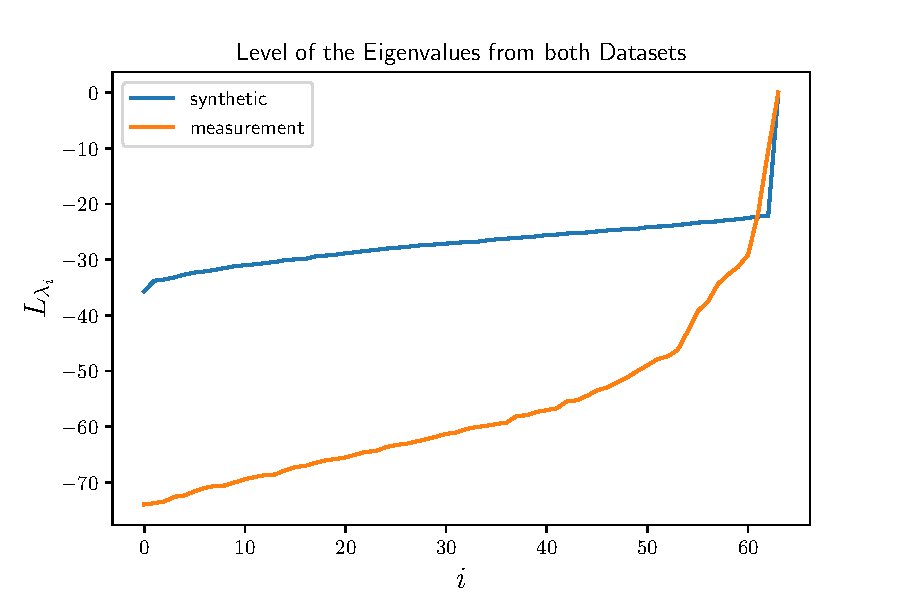
\includegraphics[width=0.9\textwidth]{figs/comparison_synthetic_measurement_data.pdf}
    \caption{Levels of the eigenvalues of a synthesized CSM (blue) and of a measured CSM (orange).}
    \label{fig:comparison_synthetic_measurement_data}    
\end{figure}

When generating the dataset, the case of a single source was considered. The audio source is located at the same position than the synthetic data, respectively to the characteristic dimension $d_m$ on the plane in front of the microphones array. The CSM are frequency dependent and the datasets consists of CSM with Helmotz number $He = 16$. Example of beamforming maps resulting from CSM from the datasets are displayed in Fig.~\ref{fig:datasets_beamforming_example} (respectively from synthetic and measurement datasets).


\begin{figure}
    \centering
    \begin{subfigure}{0.45\textwidth}
        \centering
        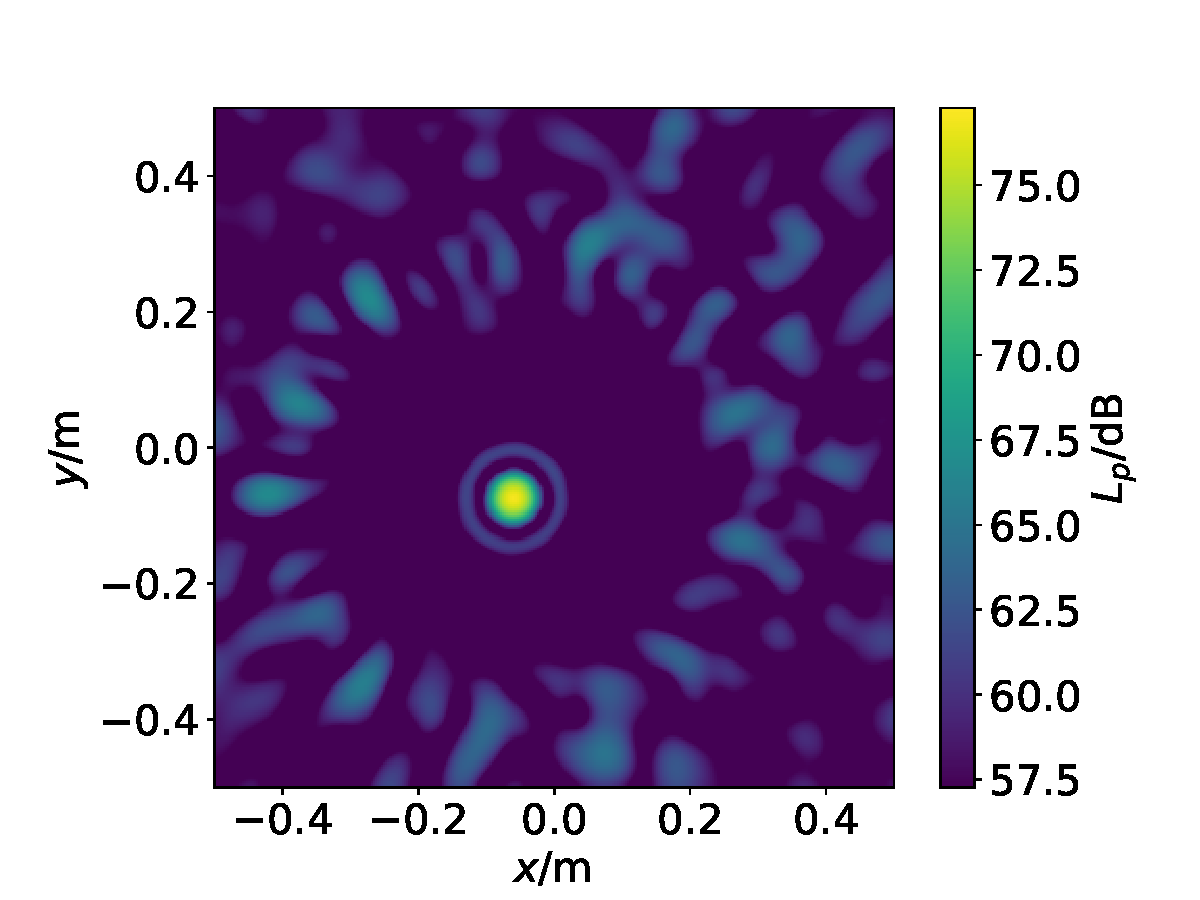
\includegraphics[width=1.3\textwidth]{figs/datasets_beamforming_example_synthetic.pdf}
        \caption{CSM from synthetic dataset}
        \label{fig:datasets_beamforming_example_synthetic}
    \end{subfigure}
    \hfill
    \begin{subfigure}{0.45\textwidth}
        \centering
        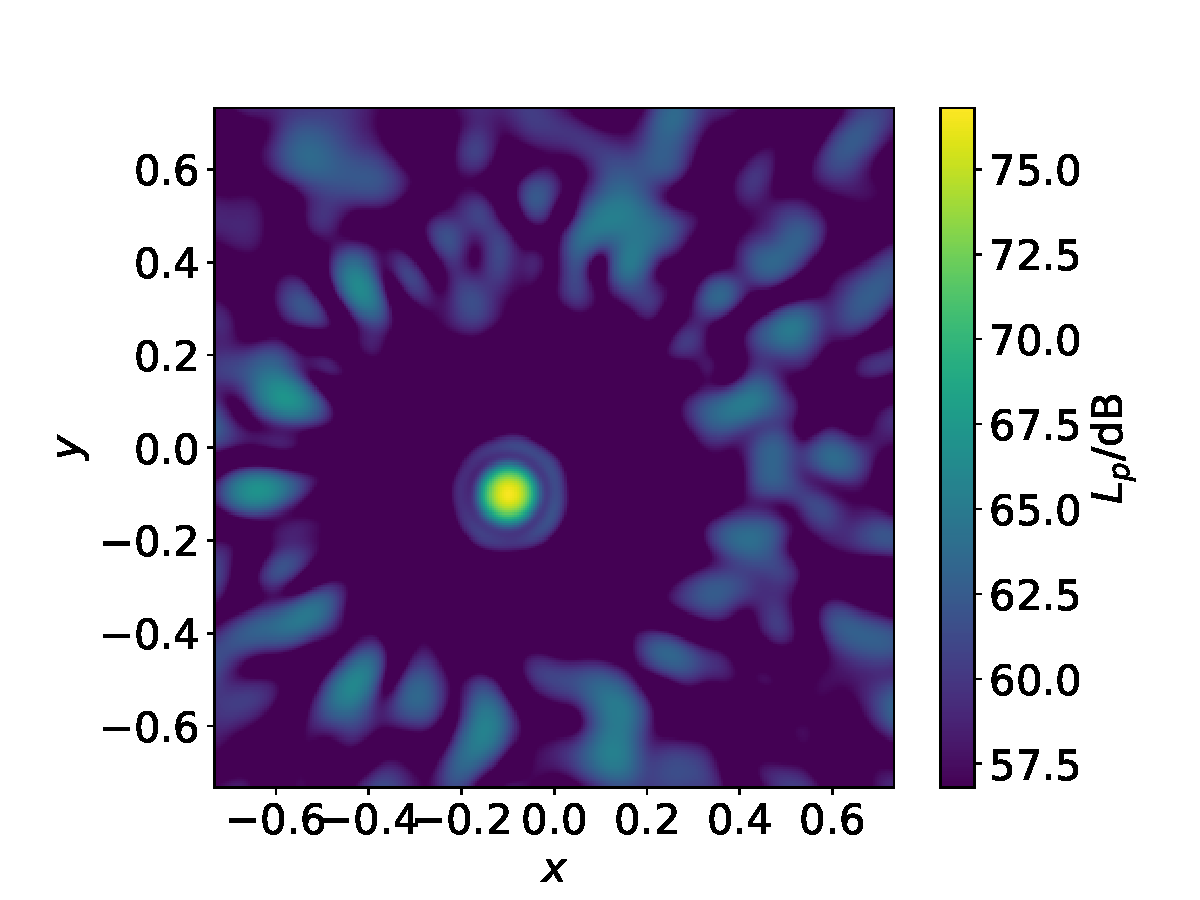
\includegraphics[width=1.3\textwidth]{figs/datasets_beamforming_example_measurement.pdf}
        \caption{CSM from measurement dataset}
        \label{fig:datasets_beamforming_example_measurement}
    \end{subfigure}
    \caption{Beamforming maps, created respectively with CSM from the synthetic dataset and from the measurement data.}
    \label{fig:datasets_beamforming_example}
\end{figure}


\section{Architectures}

In order to generate the different types of data, WGAN-GPs were designed. The different implementations were adapted from \cite{nain2020wgangp}.

\subsection{Generating Eigenvalues}

\subsubsection{Generating Scaled Eigenvalues}

The first WGAN-GP created was to generate the scaled eigenvalues $[\lambda_0, \dots, \lambda_{63}] \in ]0,1]^{64}$. These eigenvalues are sorted such that $\lambda_0 \leq \lambda_1 \leq \dots \leq \lambda_{63}$. It can be noted that the eigenvalues are real since the CSM is symmetric. Unlike in the implementation of \cite{nain2020wgangp}, when generating the eigenvalues, both inner networks (generator and critic) do not have a convolutional but a perceptron structure. A convolutional structure is relevant when the data to generate is an image. A convolutional layer is good at seeing patterns in image, by identifying topological structures in neighboring pixels.

Another changes that was made compared to the implementation of \cite{nain2020wgangp}, is that a ReLU activation function and a small positive offset noise $n = 10^{-100}$ were added as the last layer of the generator. This change was made to ensure that the generator only create positive eigenvalues. 

Finally, before being fed to the discriminator, generated eigenvalues are scaled such that $0 \leq \lambda_i \leq 1$ for $\lambda_i \in \mathbf{\lambda}$. Normalizing eigenvalues in this way is done to reduce the size of the sample space. This is illustrated in Fig.~\ref{fig:flowchart_wgangp}. Both architectures of the generator and critic used are illustrated respectively in tables Tab.~\ref{tab:evals_generator_WGANGP_architecture} and Tab.~\ref{tab:evals_critic_WGANGP_architecture}.

\begin{figure}[htb]
    \centering
    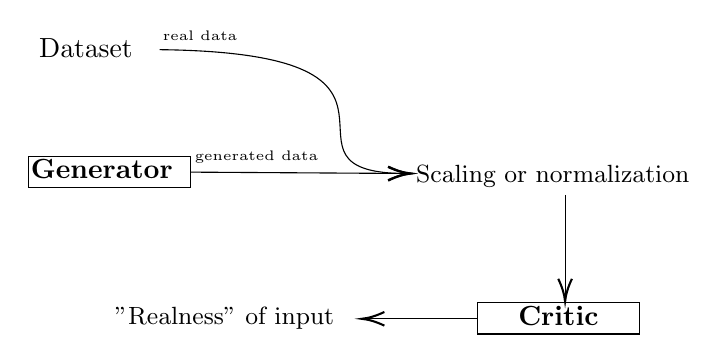
\begin{tikzpicture}[x=0.75pt,y=0.75pt,yscale=-1,xscale=1]
        %uncomment if require: \path (0,300); %set diagram left start at 0, and has height of 300
        
        %Curve Lines [id:da24102753764051987] 
        \draw    (65,9.33) .. controls (211.27,10.99) and (109.03,69.41) .. (184.84,69.01) ;
        \draw [shift={(186,69)}, rotate = 179.27] [color={rgb, 255:red, 0; green, 0; blue, 0 }  ][line width=0.75]    (10.93,-3.29) .. controls (6.95,-1.4) and (3.31,-0.3) .. (0,0) .. controls (3.31,0.3) and (6.95,1.4) .. (10.93,3.29)   ;
        %Straight Lines [id:da042737199958181704] 
        \draw    (79.67,68.33) -- (184,68.99) ;
        \draw [shift={(186,69)}, rotate = 180.36] [color={rgb, 255:red, 0; green, 0; blue, 0 }  ][line width=0.75]    (10.93,-3.29) .. controls (6.95,-1.4) and (3.31,-0.3) .. (0,0) .. controls (3.31,0.3) and (6.95,1.4) .. (10.93,3.29)   ;
        %Straight Lines [id:da48348965218999584] 
        \draw    (260.33,79.33) -- (260.33,128.67) ;
        \draw [shift={(260.33,130.67)}, rotate = 270] [color={rgb, 255:red, 0; green, 0; blue, 0 }  ][line width=0.75]    (10.93,-3.29) .. controls (6.95,-1.4) and (3.31,-0.3) .. (0,0) .. controls (3.31,0.3) and (6.95,1.4) .. (10.93,3.29)   ;
        %Straight Lines [id:da6843336271870258] 
        \draw    (218,139) -- (164.33,139) ;
        \draw [shift={(162.33,139)}, rotate = 360] [color={rgb, 255:red, 0; green, 0; blue, 0 }  ][line width=0.75]    (10.93,-3.29) .. controls (6.95,-1.4) and (3.31,-0.3) .. (0,0) .. controls (3.31,0.3) and (6.95,1.4) .. (10.93,3.29)   ;
        %Shape: Rectangle [id:dp5961208628096415] 
        \draw   (1.67,60.67) -- (79.67,60.67) -- (79.67,75.67) -- (1.67,75.67) -- cycle ;
        %Shape: Rectangle [id:dp7837205891485919] 
        \draw   (218.33,131.33) -- (296.33,131.33) -- (296.33,146.33) -- (218.33,146.33) -- cycle ;
        
        % Text Node
        \draw (1.67,61) node [anchor=north west][inner sep=0.75pt]   [align=left] {\textbf{Generator}};
        % Text Node
        \draw (236.5,131.75) node [anchor=north west][inner sep=0.75pt]   [align=left] {\textbf{Critic}};
        % Text Node
        \draw (5.67,2.67) node [anchor=north west][inner sep=0.75pt]   [align=left] {Dataset};
        % Text Node
        \draw (187.33,63.67) node [anchor=north west][inner sep=0.75pt]   [align=left] {{\small Scaling or normalization}};
        % Text Node
        \draw (80.67,56.67) node [anchor=north west][inner sep=0.75pt]   [align=left] {{\tiny generated data}};
        % Text Node
        \draw (65.33,-1) node [anchor=north west][inner sep=0.75pt]   [align=left] {{\tiny real data}};
        % Text Node
        \draw (42.33,132) node [anchor=north west][inner sep=0.75pt]   [align=left] {{\small "Realness" of input}};    
    \end{tikzpicture}
    \caption{Full structure of the implementation used in the WGAN-GP to generate eigenvalues or eigenvectors. The eigenvalues are being scaled before being fed to the generator, while the eigenvectors are being normalized.}
    \label{fig:flowchart_wgangp}
  \end{figure}



\subsubsection{Generating the Levels of Scaled Eigenvalues}

Another approach to generate the scaled eigenvalues $\lambda_0, \dots, \lambda_{63}$ was to generate them from their level values $ L_{\lambda_0} , \dots,  L_{\lambda_{63}} $. The levels are computed with:

\begin{equation}
    L_{\lambda_i} = 10 \log_{10}(\frac{\lambda_i}{\lambda_{63}})
\end{equation}

where $\lambda_{63}$ is the strongest eigenvalue. Since all values $L_{\lambda_i}$ are non-positive, the generator has been built such that the two last steps are first a ReLU, followed by a multiplication by $-1$. This way it can be ensured that the network only produces non-positive spectrum. This approach was also justified by the usage of Leaky ReLU as activation throughout the generator. 

Because Leaky ReLU were also used in the critic, the first layer of its network is also a multiplicative layer. Therefore, the critic is not trained to detect real from fake levels, but rather real from fake negative levels, which is equivalent. 

The architectures used for the generator and the critic are shown respectively in Tab.~\ref{tab:evals_dB_generator_WGANGP_architecture} and Tab.~\ref{tab:evals_dB_critic_WGANGP_architecture}.


\subsection{Generating Eigenvectors}

In order to generate the eigenvector, it was decided to start by only generating the eigenvector corresponding to the strongest eigenvalue, as a proof of concept. This eigenvector was defined as main eigenvector. Indeed, using equation \ref{rank_I_csm}, once a main eigenvector is produced, its quality can be directly assessed by computing a Rank I CSM, allowing to perform beamforming and locate the source position. In Fig.~\ref{fig:measurement_sample_rank_I_beamforming}, a beamforming map, created with a rank I CSM obtained from measurement data is showed.

\begin{figure}
    \centering
    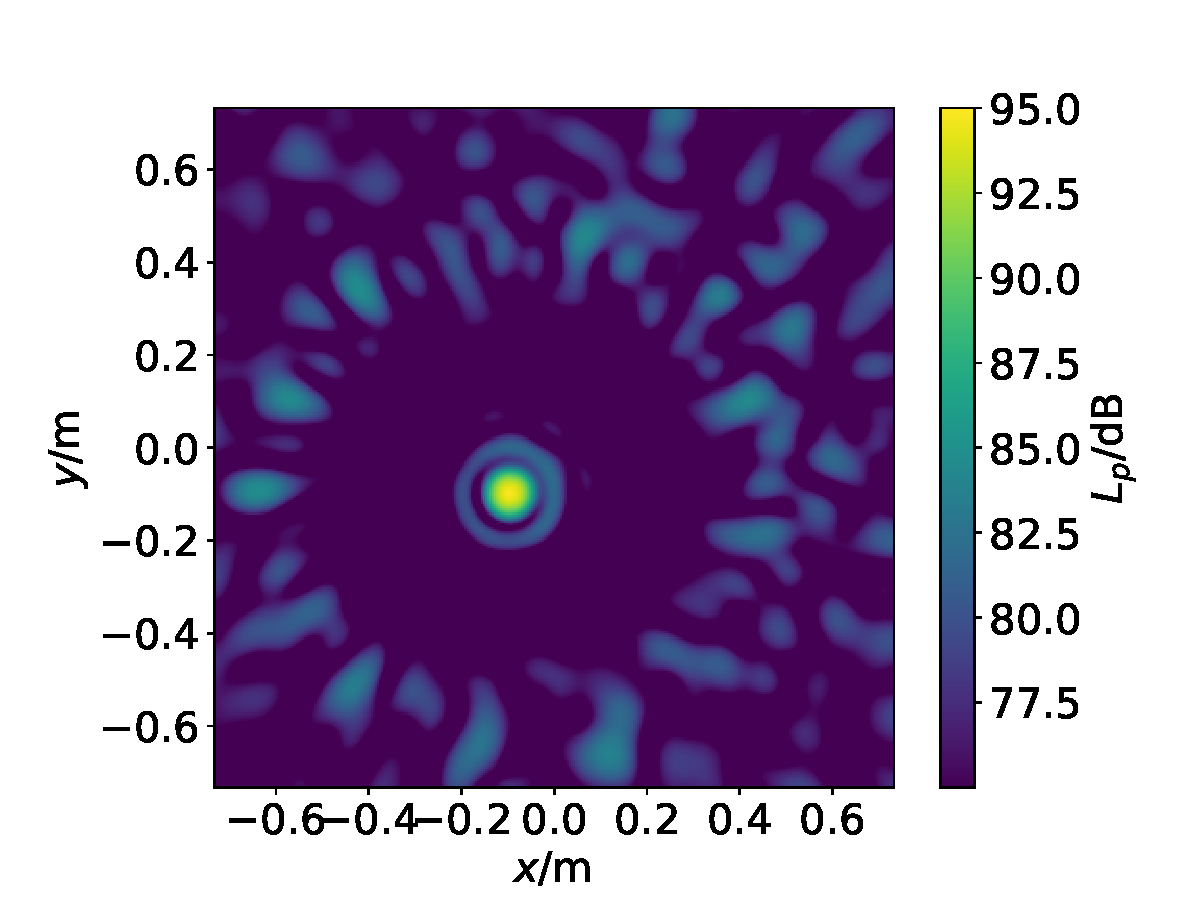
\includegraphics[width=0.8\textwidth]{figs/measurement_sample_rank_I_beamforming.pdf}
    \caption{Beamforming map, created with a rank I CSM created from measurement data}
    \label{fig:measurement_sample_rank_I_beamforming}
\end{figure}



Moreover, first generating only the main eigenvector can be justified by the fact, it is the most meaningful eigenvector. Indeed, each eigenvector belongs to a different incoherent source. If there would to be  multiple coherent source, all the energy and their position merges into a single eigenmode. Since the case where there is only one source is under consideration, only the eigenvector with the biggest index corresponds to a DoA/source and the remaining 63 eigenvectors corresponds to noise.  

In Fig.~\ref{fig:histograms_eigenvectors} are plotted the histograms of the values of the scalars of the eigenvectors with different index. It can be noticed that the values of the eigenvectors with low index seem to follow a Gaussian distribution, whereas the values of the eigenvectors with index close to the maximal index are following a more complex distribution.

\begin{figure}
    \centering
    \makebox[\textwidth][c]{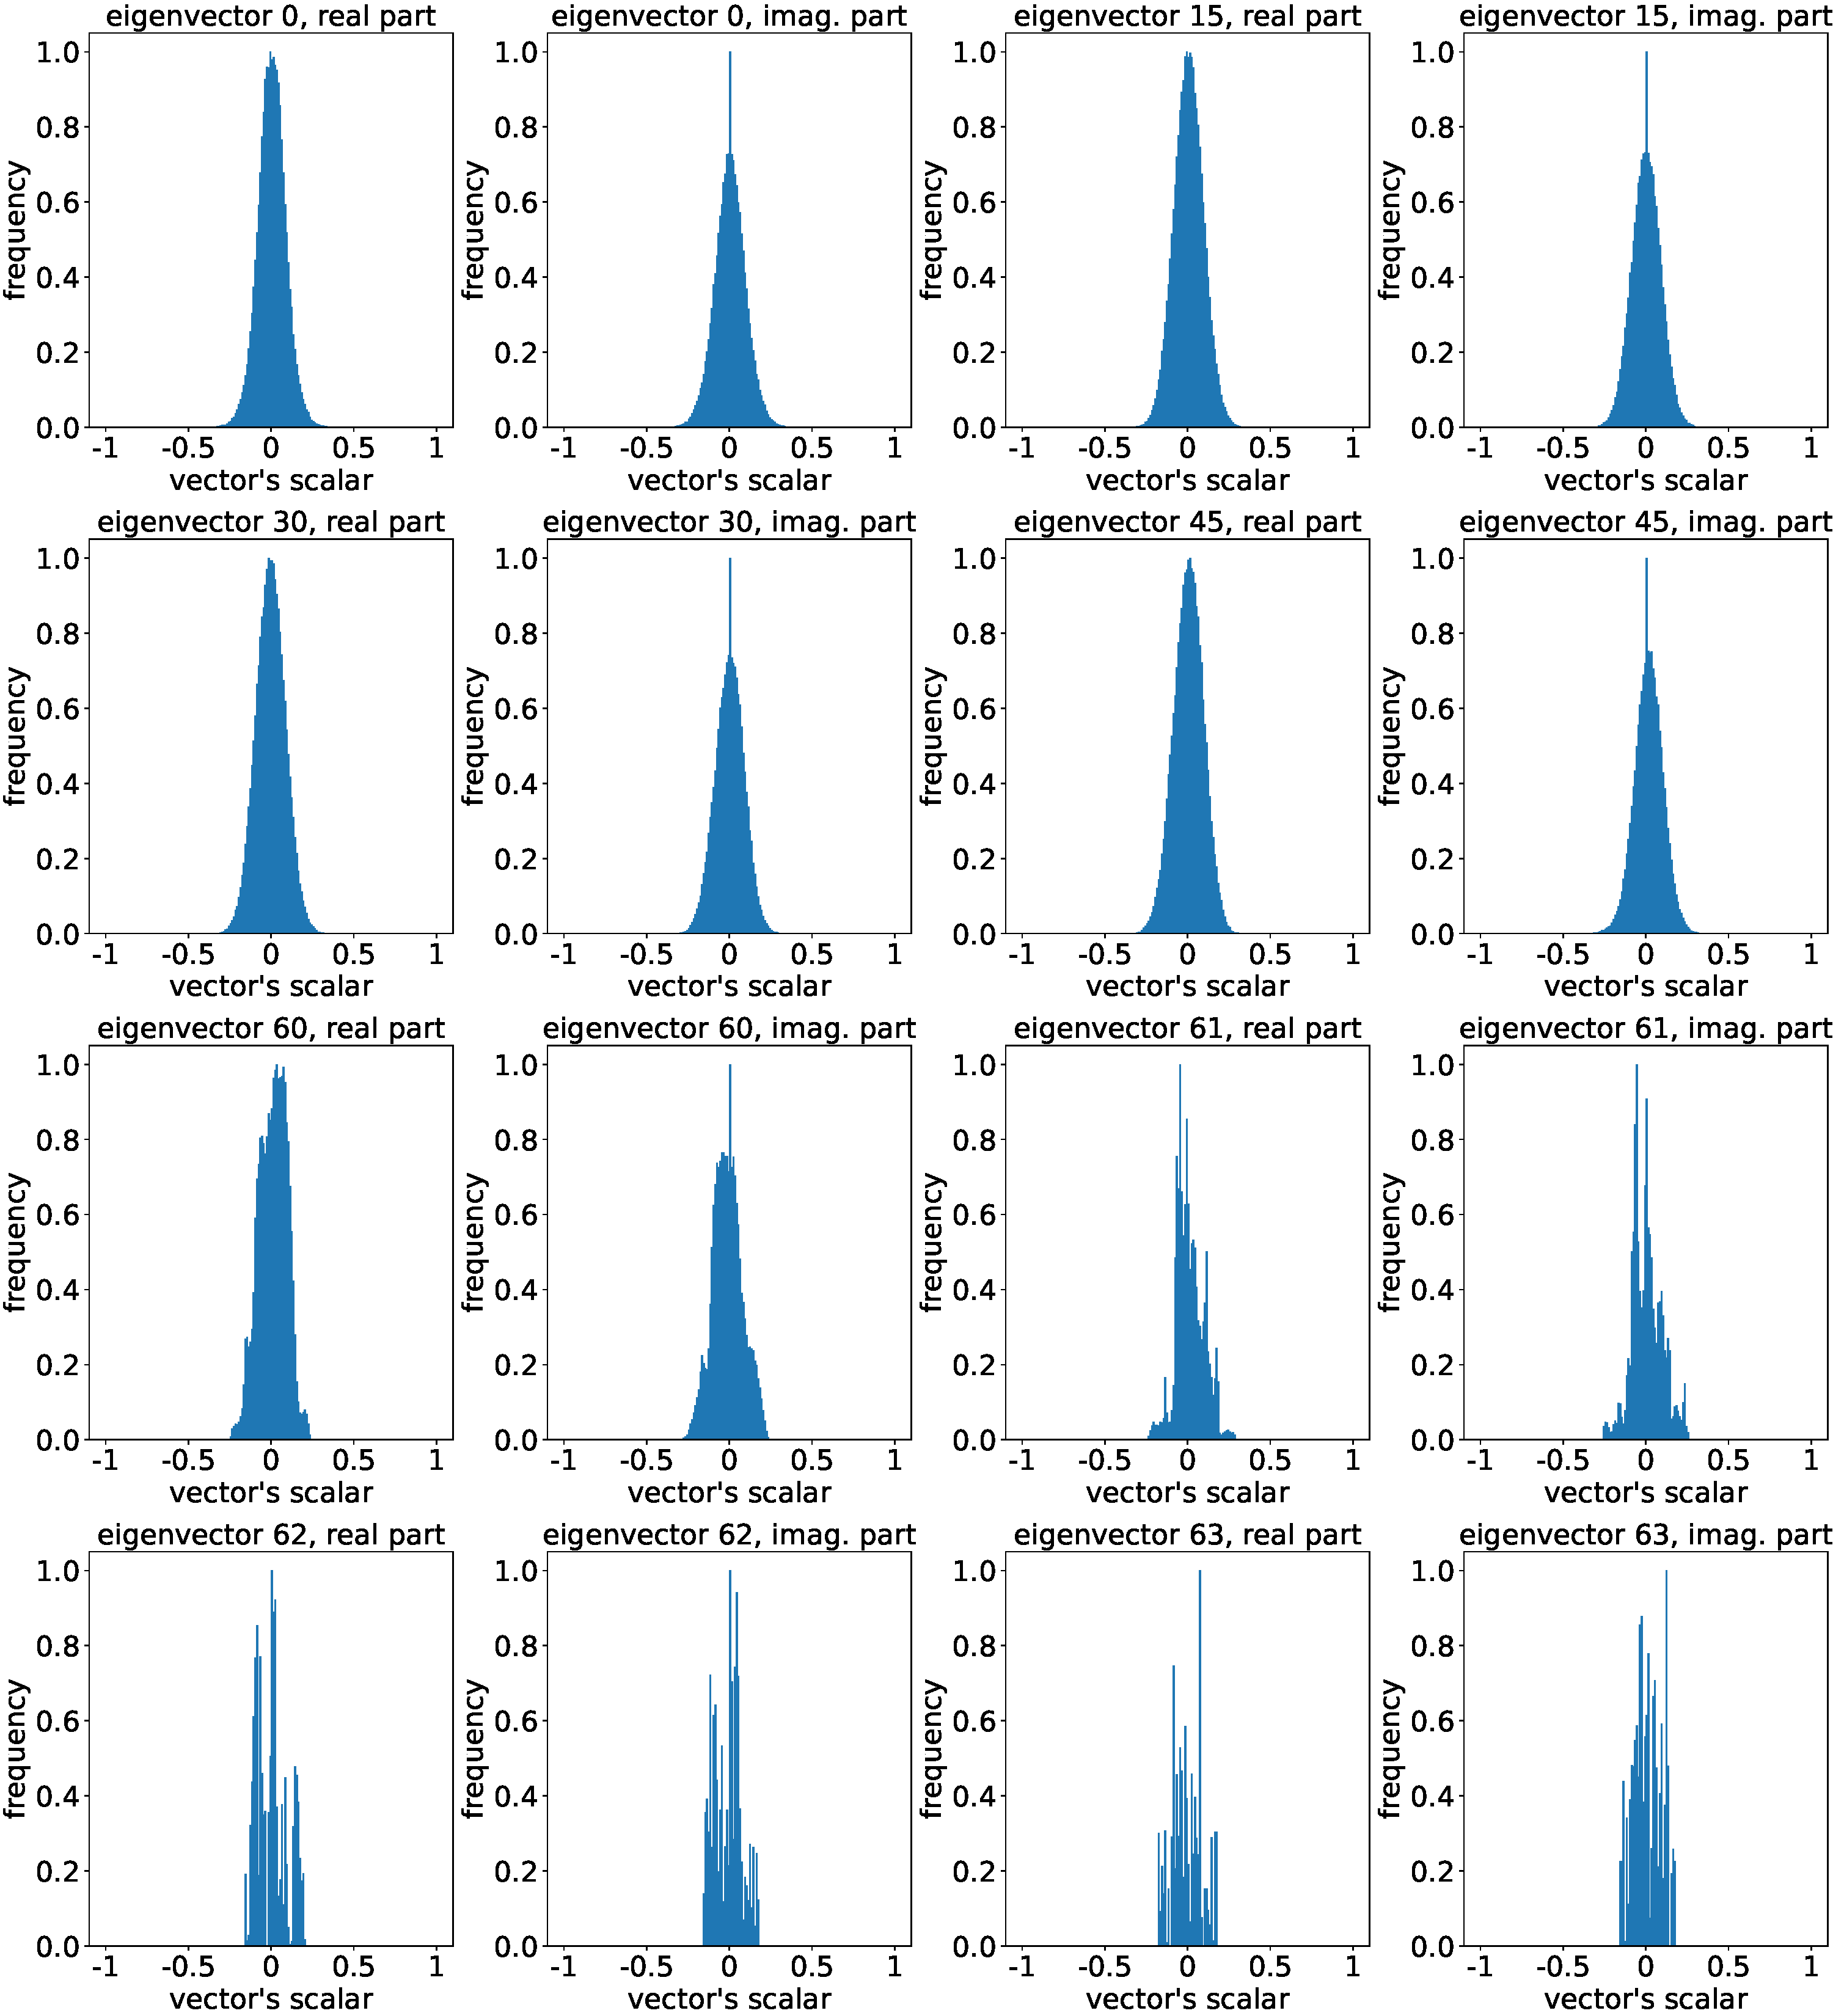
\includegraphics[width=1.2\textwidth]{figs/histograms_eigenvectors.pdf}}
    \caption{Histograms of the values of the scalars of the eigenvectors with different index. The eigenvector with index $63$ is the main eigenvector (two last histograms).}
    \label{fig:histograms_eigenvectors}
\end{figure}

\subsubsection{Main Eigenvector}

Since the main eigenvector is $\in \mathbb{C}^{64}$, a network with a similar architecture as the one used for the eigenvalues can be used. But instead of scaling the generated sample, they are normalized before being fed to the discriminator. Here by normalization is meant that the main eigenvector is recomputed such that its direction remains the same but its norm is equal to 1. Since the main eigenvector is complex, it is fed to the network as a concatenation of its real and imaginary part, namely as a vector $\in \mathbb{R}^{128}$. The full WGAN-GP structure is illustrated in Fig.~\ref{fig:flowchart_wgangp}. The architectures both the generator and critic are illustrated respectively in the tables Tab.~\ref{tab:main_evec_generator_WGANGP_architecture} and Tab.~\ref{tab:main_evec_critic_WGANGP_architecture}.


\section{Data Augmentation}

\subsection{Using Generated Eigenvalues}

An idea for augmenting datasets of CSM of recorded pressure vectors $\mathbf{p} \mathbf{p}^H$ is introduced. For a received synthetic CSM $\mathbf{\hat{C}}$, its  eigendecomposition $\mathbf{\hat{C}} = \mathbf{V} \mathbf{\Lambda} \mathbf{V}^H$ is computed The eigenvalues diagonal matrix $ \mathbf{\Lambda}$ is then replaced by eigenvalues $\hat{\mathbf{\Lambda}}$ generated using a WGAN-GP, providing with semi-generated CSM:

\begin{equation}
    \mathbf{\hat{C}}_\text{augm.}  = \mathbf{V} \hat{\mathbf{\Lambda}} \mathbf{V}^H
\end{equation}

\subsection{Using Generated Main Eigenvector}

A similar idea can be performed, but this time replacing the main eigenvector in the eigendecomposition of a synthetic CSM, by a main eigenvector generated by a WGAN-GP. Formally, in the eigendecomposition $\mathbf{\hat{C}} = \mathbf{V} \mathbf{\Lambda} \mathbf{V}^H$, the vector matrix $\mathbf{V} = [\mathbf{v}_1^T, \dots, \mathbf{v}_M^T]$, is replaced by a matrix $\hat{\mathbf{V}} = [\mathbf{v}_1^T, \dots, \hat{\mathbf{v}}_M^T]$, where $\hat{\mathbf{v}}_M$ is a main eigenvector generated by a WGAN-GP. The semi-generated CSM is then:

\begin{equation}
    \mathbf{\hat{C}}_\text{augm.}  = \hat{\mathbf{V}} \mathbf{\Lambda} \hat{\mathbf{V}}^H
\end{equation}



\section{Parameters}

The WGAN-GP for generating the scaled eigenvalues, the level of eigenvalues and the main eigenvectors all used the same parameters. The batch size was set to $16$ and the latent dimension to $128$. The optimizers used both for the critic and generator are Adam optimizers with a learning rate $lr=0.0002$, $\beta_1=0.5$ and $\beta_2=0.9$. Every time the generator was trained once, the critic was trained 3 times (i.e $n_{critic} = 3$). The weight of the gradient penalty is equal to $10$. All three WGAN-GP were trained on the same GPU, namely a NVIDIA GeForce RTX 3090. When performing the training, the training setup was different for the three models, namely:

\begin{itemize}
    \item For training the WGAN-GP for generating the scaled eigenvalues, the initial training consisted of 100 epochs, with 1 step per epoch and the fine-tuning of 200 epochs, with 5 steps per epoch.
    \item For training the WGAN-GP for generating the level of eigenvalue, the initial training consisted of 100 epochs, with 1 step per epoch and the fine-tuning of 120 epochs, with 1 steps per epoch
    \item For training the WGAN-GP for generating the main eigenvector, The initial training consisted of 500 epochs, with 1 step per epoch and the fine-tuning of 200 epochs, with 1 steps per epoch.
\end{itemize}

\chapter{Results}

\section{Generating Eigenvalues} 

\subsection{Generating Eigenvalues from their Scaled Values}

In Fig.~\ref{fig:loss_evals_wgangp}  is displayed the loss function when respectively training with the synthetic data and fine-tuning with measurement data. Only the loss function of the critic is displayed, since it is the only one relevant to assess convergence of a WGAN-GP (see Section~\ref{sec:assessing_perf}). Training the WGAN-GP took 19s for the initial training and 10s for the fine-tuning. It can be observed that the model converged before the fine-tuning. The critic's loss first shows a steep decrease before making its way up to zero. This means that the distribution of the real samples and generated ones are really close to each other, with respect to the Wasserstein distance. During the fine-tuning, the loss remained close to zero, hinting that little weight updates were required in order to generate measurement data. It can be observed that there was more epoch for fine-tuning than for the initial training. This design choice was made to ensure the WGAN-GP would converge again during fine-tuning, but it can be observed from the behavior of the loss that it was not necessary and that 50 epochs would have been sufficient for fine-tuning.    

\begin{figure}
    \centering
    \makebox[\textwidth][c]{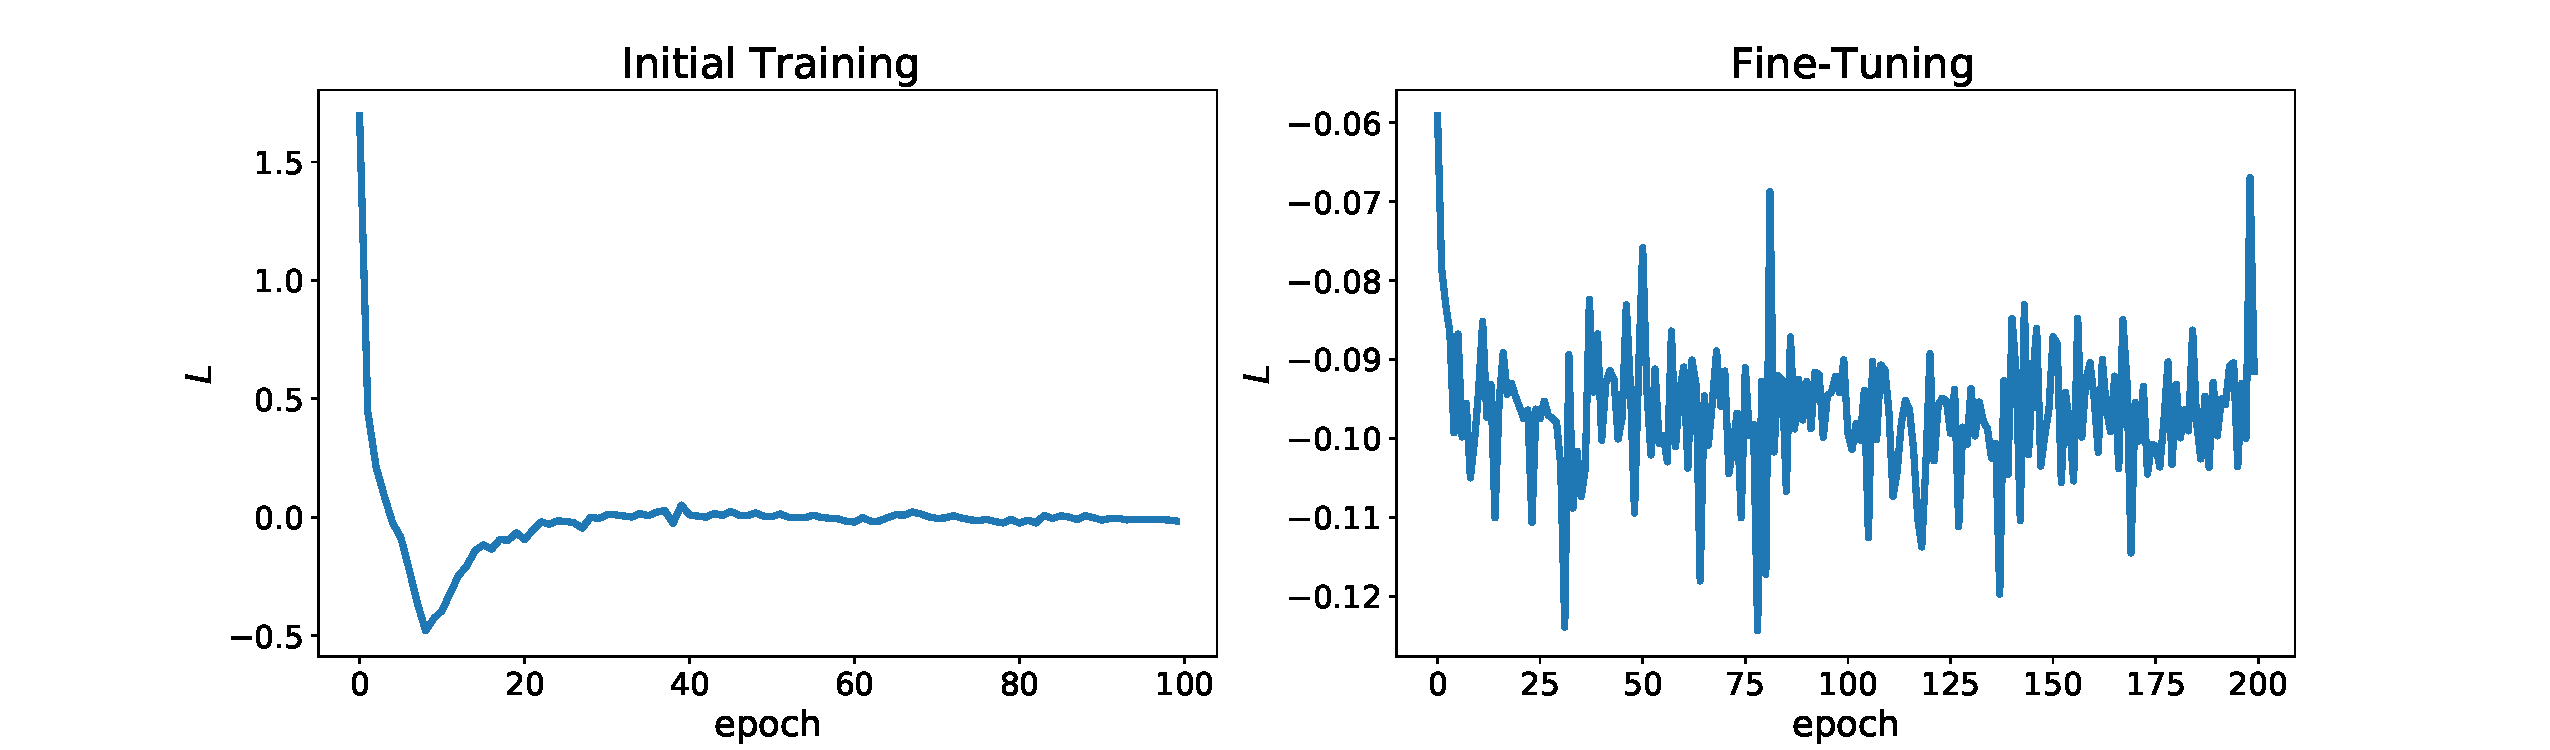
\includegraphics[width=1.2\textwidth]{figs/loss_evals_wgangp.pdf}}
    \caption{The loss functions of the critic of the WGAN-GP for eigenvalues generation, respectively while performing the initial training and while fine-tuning}
    \label{fig:loss_evals_wgangp}
\end{figure}

In Fig.~\ref{fig:samples_evals_wgangp}, a comparison between real and generated eigenvalues is displayed. It contains an example eigenvalues from the synthetic dataset (green), an example of eigenvalues from the measurement dataset (red), sample eigenvalues generated by the WGAN-GP before the fine-tuning (blue) and sample eigenvalues generated by the WGAN-GP after fine-tuning (orange). All those quantities are displayed as their levels values. It can be observed that both the samples generated before and after fine-tuning show a sudden and steep drop in value, reaching a level around $10^{-100}$.

\begin{figure}
    \centering
    \makebox[\textwidth][c]{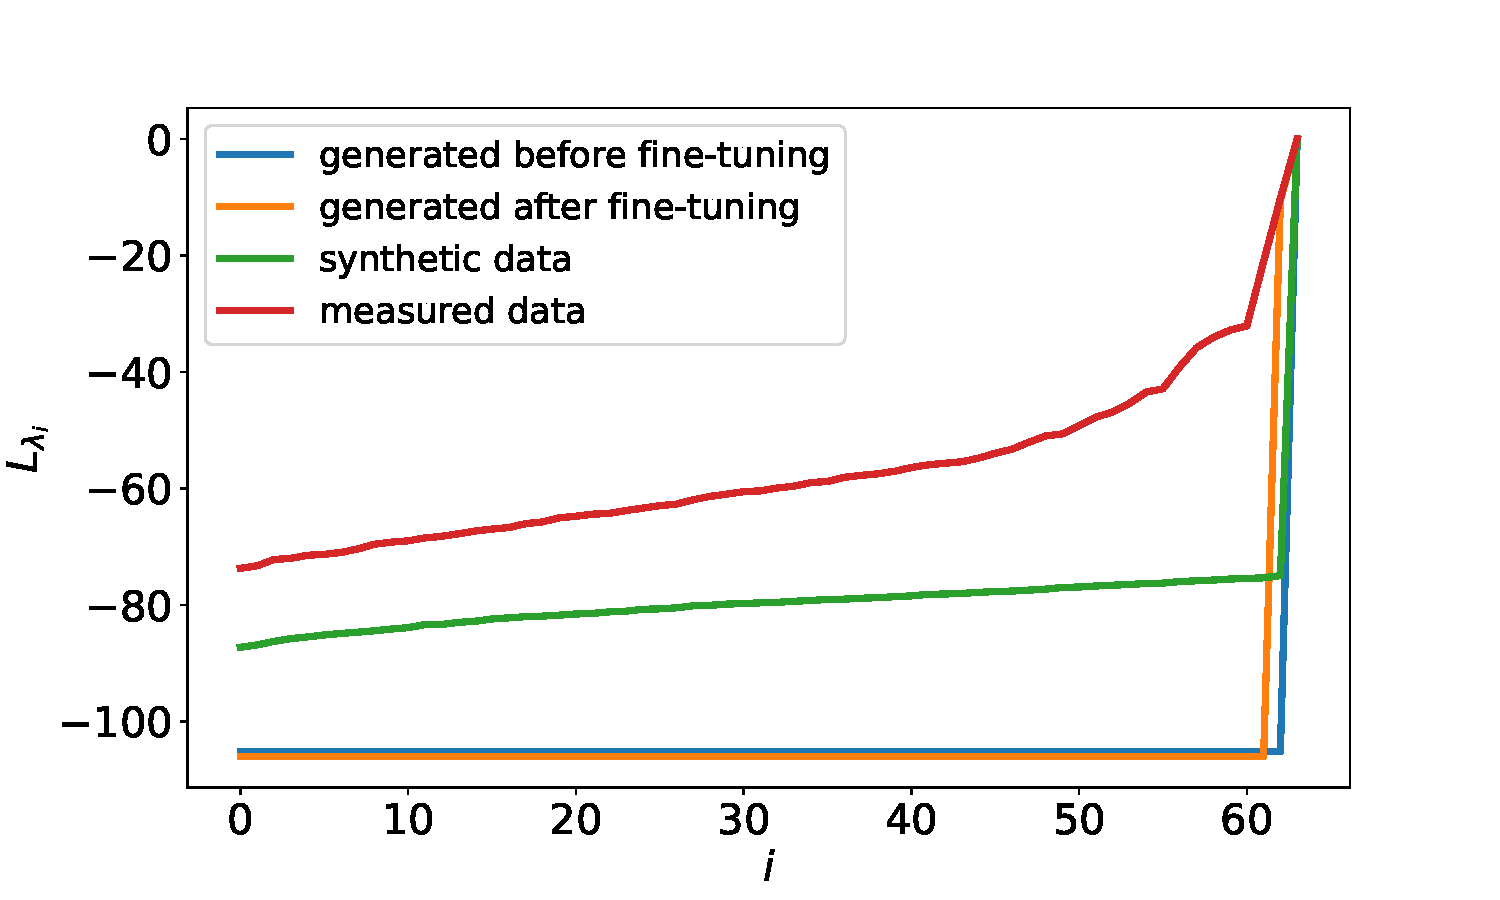
\includegraphics[width=0.8\textwidth]{figs/samples_evals_wgangp.pdf}}
    \caption{This graph shows the level of eigenvalues of a synthetic CSM (green), level of eigenvalues of a measured CSM (red), level of eigenvalues generated with the WGAN-GP for scaled eigenvalues after the initial training (blue) and level of eigenvalues generated with the WGAN-GP for scaled eigenvalues after the fine-tuning (orange).}
    \label{fig:samples_evals_wgangp}
\end{figure}

\subsection{Generating Eigenvalues from their Level Values}

The losses during training of the critic of the WGAN-GP for generating eigenvalues from their level values are displayed in Fig.~\ref{fig:loss_evals_dB_wgangp}. Training the WGAN-GP took 19s for the initial training and 1.9s for the fine-tuning. It can be seen that the model converged before fine-tuning. Then, during the fine-tuning, the loss drops before converging again.

\begin{figure}
    \centering
    \makebox[\textwidth][c]{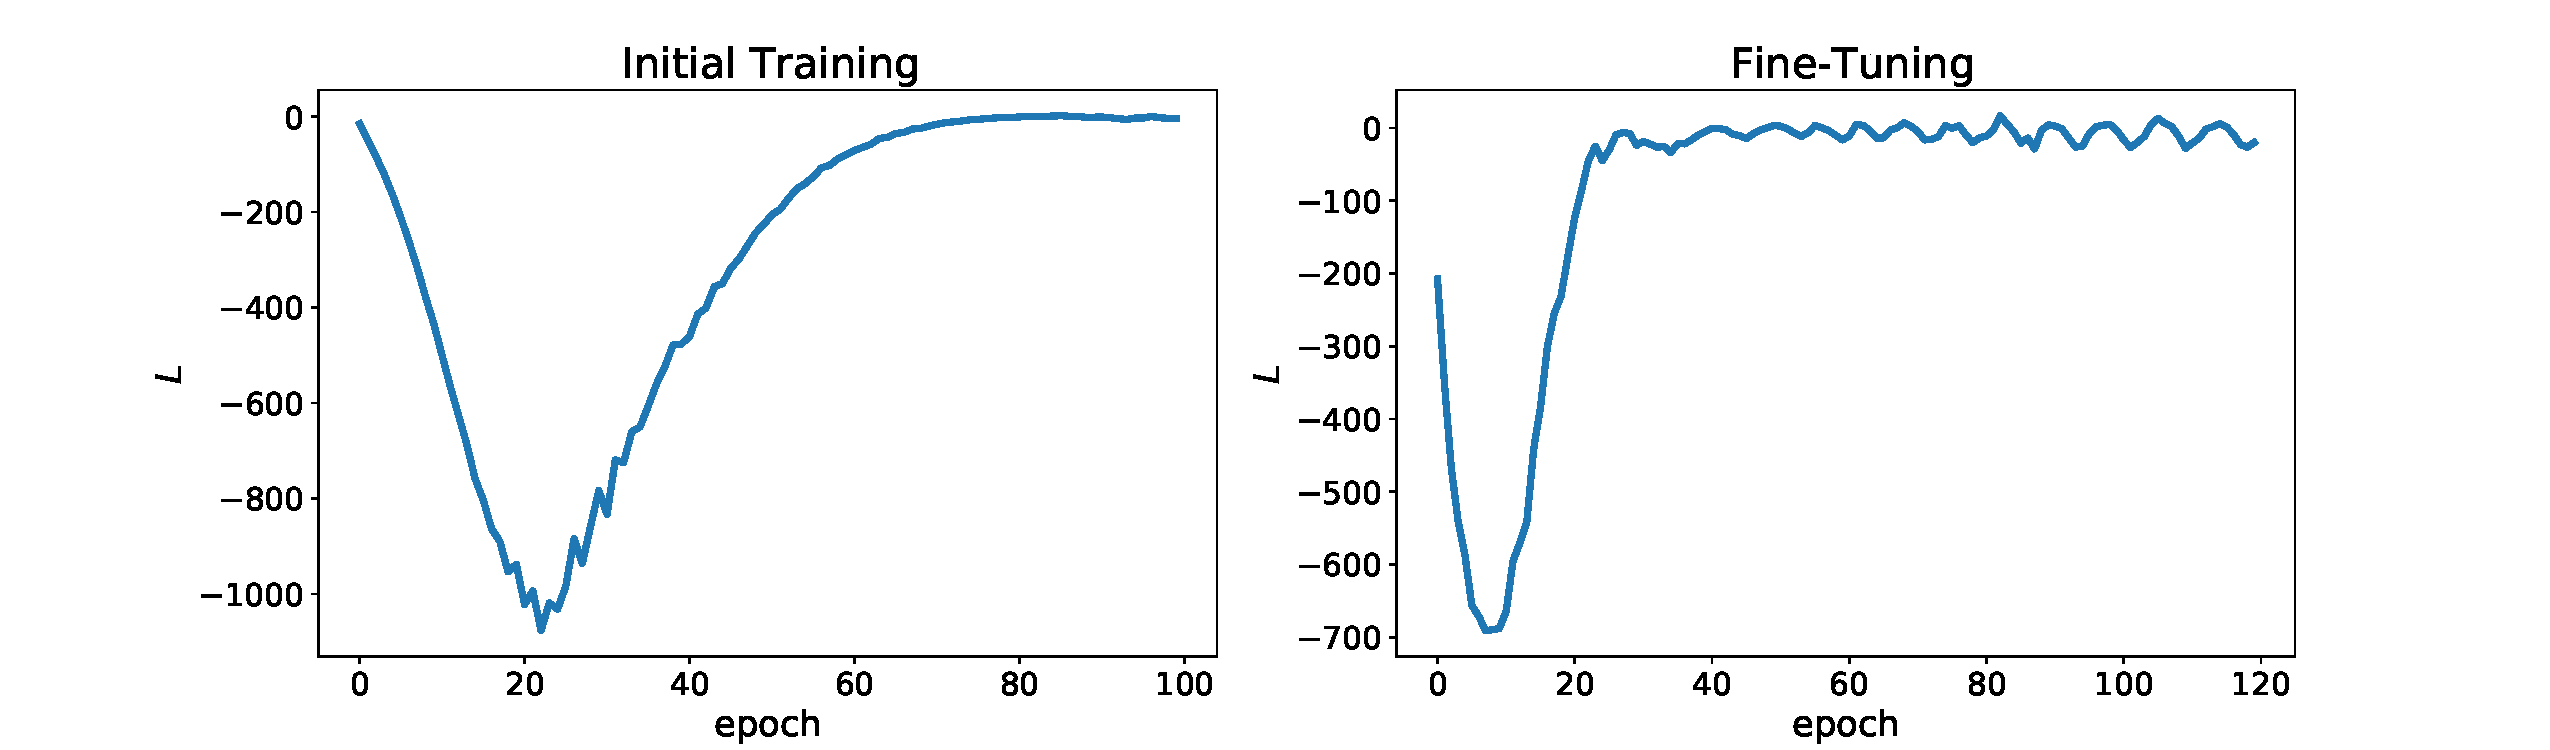
\includegraphics[width=1.2\textwidth]{figs/loss_evals_dB_wgangp.pdf}}
    \caption{The loss functions of the critic of the WGAN-GP for the levels of eigenvalues generation, respectively while performing the initial training and while fine-tuning}
    \label{fig:loss_evals_dB_wgangp}
\end{figure}


In Fig.~\ref{fig:samples_evals_dB_wgangp} is displayed a comparison between levels of the eigenvalues from the synthetic dataset (green), levels of the eigenvalues from the measurement dataset (red), sample levels of eigenvalues generated by the WGAN-GP before fine-tuning (blue) and sample levels of eigenvalues generated by the WGAN-GP after fine-tuning (orange). It can be seen that the sample generated before fine-tuning follows quite well the levels from the synthetic dataset, though not decaying as linearly. The sample generated after fine-tuning display a similar decay as the levels from the measurement dataset.

\begin{figure}
    \centering
    \makebox[\textwidth][c]{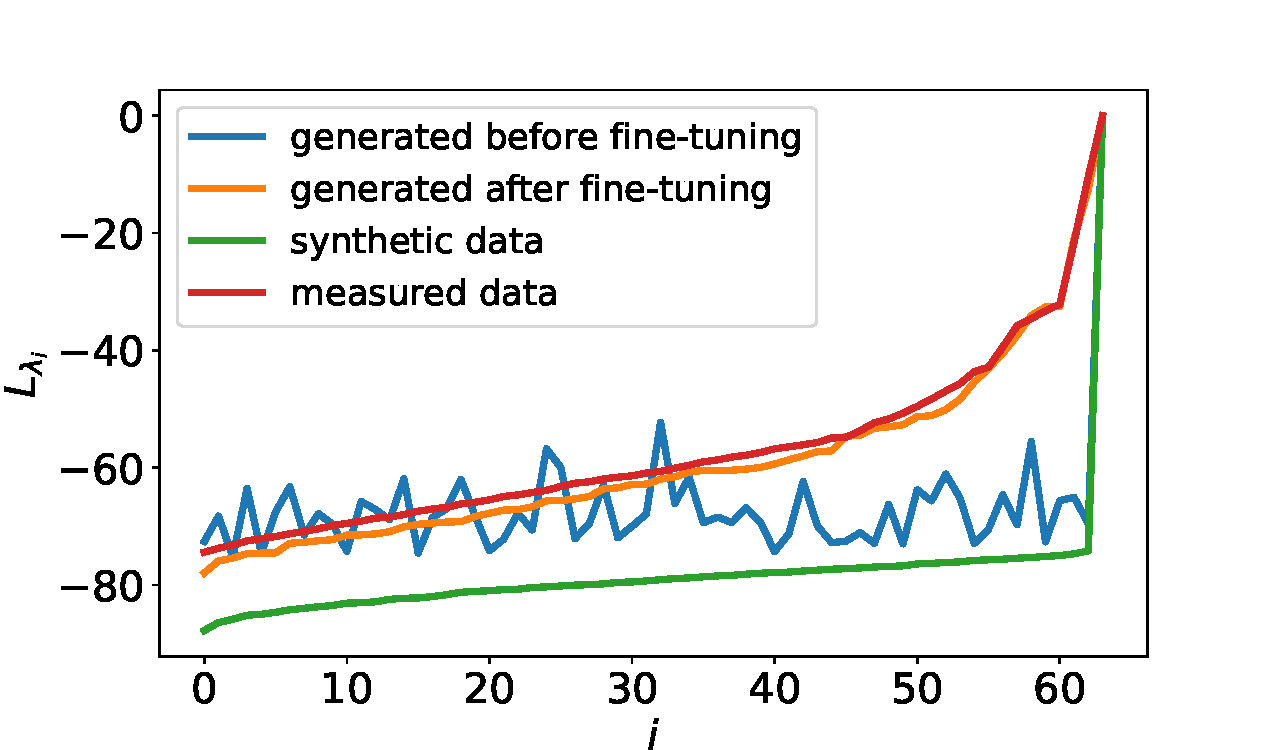
\includegraphics[width=0.8\textwidth]{figs/samples_evals_dB_wgangp.pdf}}
    \caption{The first graph shows levels of eigenvalues of a synthetic CSM (green), levels of eigenvalues of a measured CSM (red), levels of eigenvalues generated with the WGAN-GP for level of eigenvalues after the initial training (blue) and levels of eigenvalues generated with the WGAN-GP for level of eigenvalues after the fine-tuning (orange).}
    \label{fig:samples_evals_dB_wgangp}
\end{figure}

In Fig.~\ref{fig:outliers_evals_dB_wgangp} is displayed a statistical study of the generated level of eigenvalues. The average generated level eigenvalues (bold) as well as the 5\% and 95\% percentiles (dotted) are showed in blue. In orange is showed the levels of eigenvalues that was used for fine-tuning. In gray are showed, for comparison purpose, the levels of eigenvalues that were not used to train this model for fine-tuning. It can be observed that the generated levels have a larger span than the measured levels of eigenvalues is almost constant, whether used for training or not. Even though the scaling is not identical between measured and generated, the eigenvalues are decaying similarly.

\begin{figure}
    \centering
    \makebox[\textwidth][c]{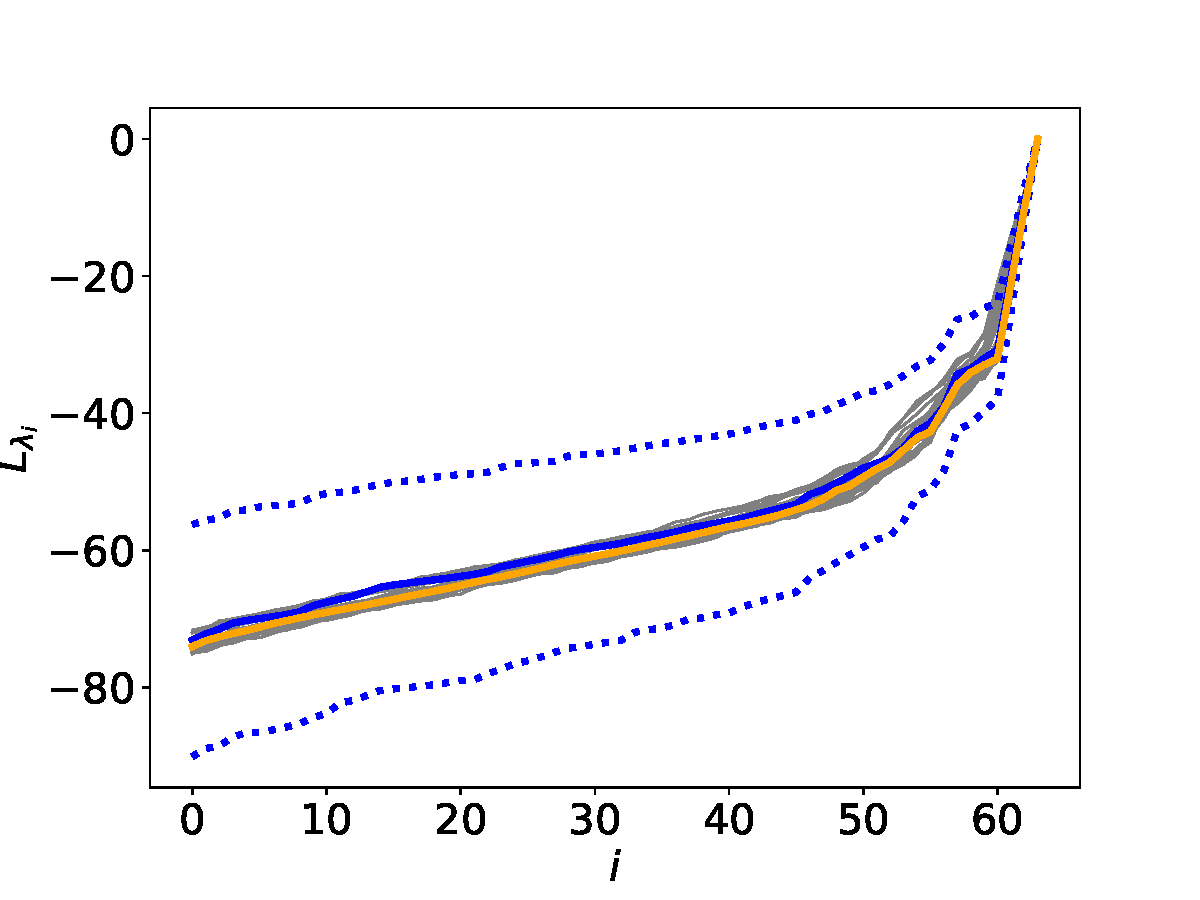
\includegraphics[width=0.8\textwidth]{figs/outliers_evals_dB_wgangp.pdf}}
    %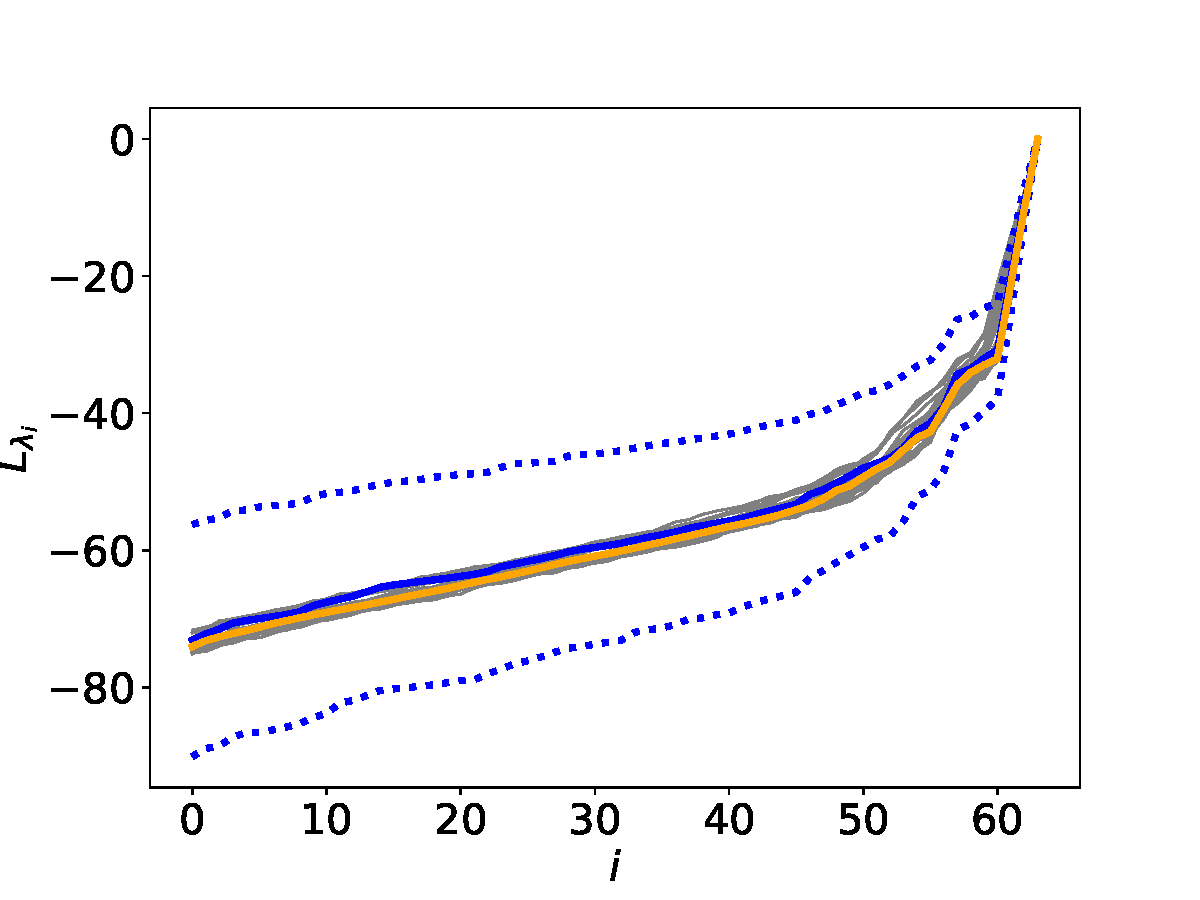
\includegraphics[width=0.9\textwidth]{figs/outliers_evals_dB_wgangp.pdf}
    \caption{In orange are displayed the level eigenvalues of the measurement CSM. In blue, the average (bold), the 5\% and 95\%percentiles (dotted) of generated level of eigenvalues are displayed. In gray are displayed examples of eigenvalues' levels coming from other measurements not used for training.}
    \label{fig:outliers_evals_dB_wgangp}    
\end{figure}

\subsection{Data Augmentation}

Fig.~\ref{fig:data_augmentation_evals} shows three different beamforming map. Fig.~\ref{fig:data_augmentation_evals_synthetic}, Fig.~\ref{fig:data_augmentation_evals_measurement} and Fig.~\ref{fig:data_augmentation_evals_augmented_csm} show respectively the beamforming map obtained when using a synthetic CSM, a measured CSM and a CSM augmented with eigenvalues. It can be observed that the map issued from an augmented CSM is closer to the map issued from a synthetic CSM.

\begin{figure}
    \centering
    \begin{subfigure}{0.45\textwidth}
        \centering
        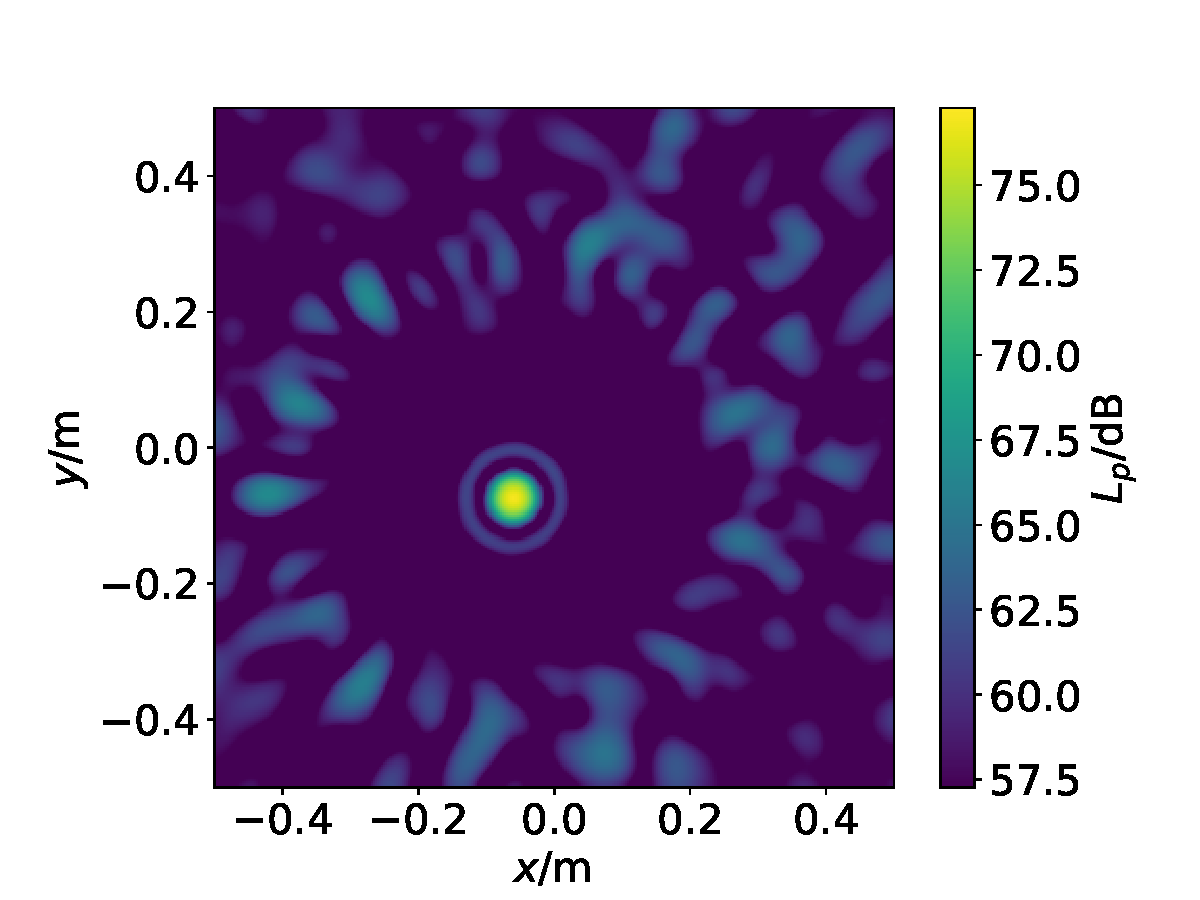
\includegraphics[width=1.3\textwidth]{figs/datasets_beamforming_example_synthetic.pdf}
        \caption{CSM from synthetic dataset}
        \label{fig:data_augmentation_evals_synthetic}
    \end{subfigure}
    \hfill
    \begin{subfigure}{0.45\textwidth}
        \centering
        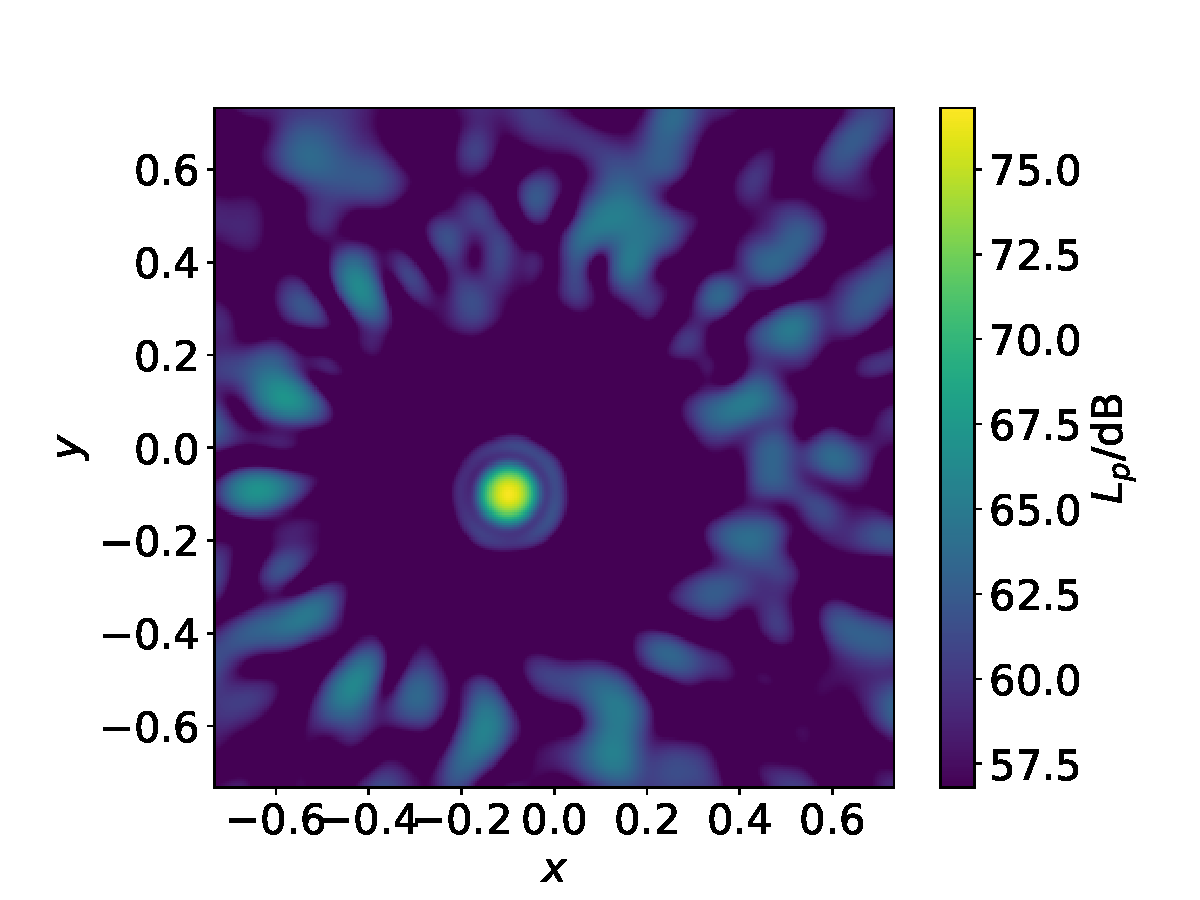
\includegraphics[width=1.3\textwidth]{figs/datasets_beamforming_example_measurement.pdf}
        \caption{CSM from measurement dataset}
        \label{fig:data_augmentation_evals_measurement}
    \end{subfigure}
    \hfill
    \begin{subfigure}{0.45\textwidth}
        \centering
        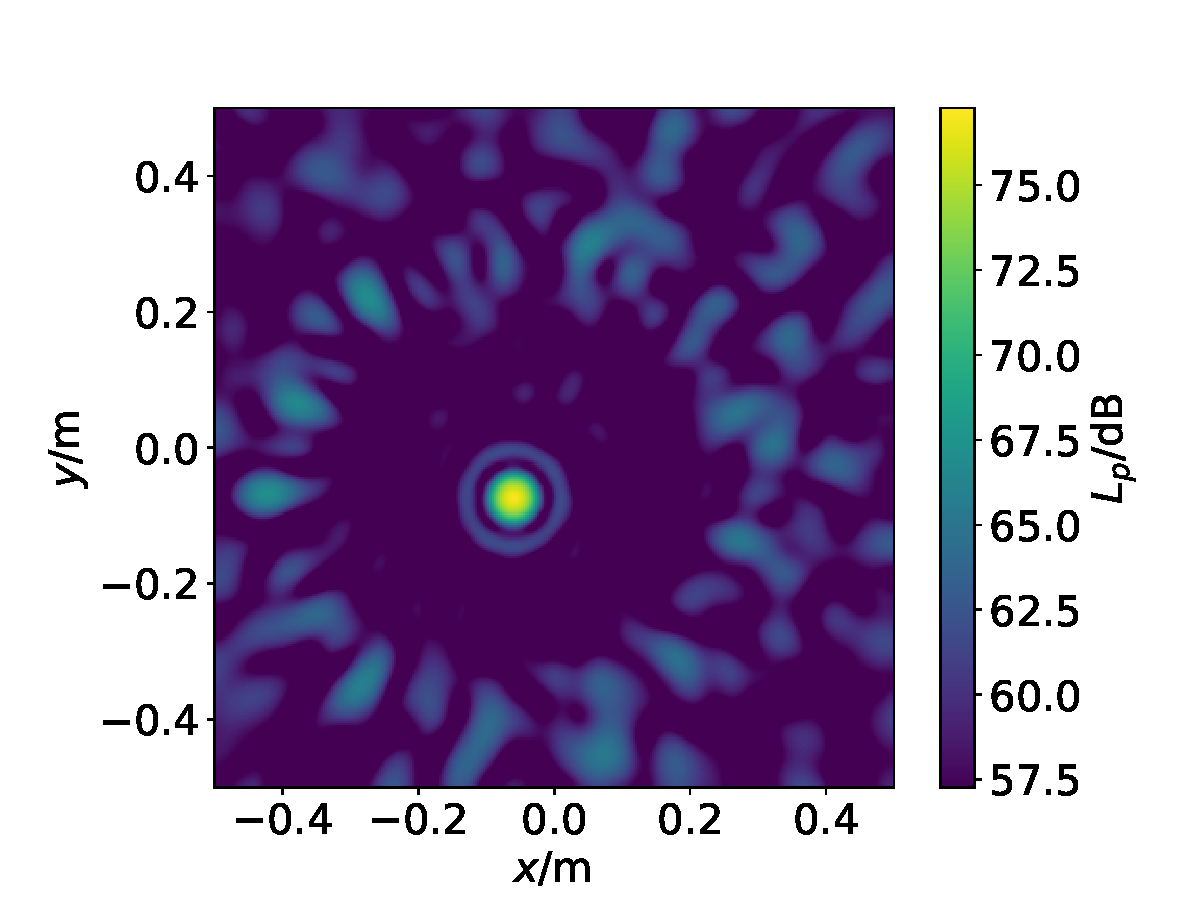
\includegraphics[width=1.3\textwidth]{figs/data_augmentation_evals_augmented_csm.pdf}
        \caption{CSM Augmented with generated eigenvalues.} 
        \label{fig:data_augmentation_evals_augmented_csm}
    \end{subfigure}
            
    \caption{Three beamforming maps obtained from synthetic CSM, measured CSM and CSM augmented with generated eigenvalues}
    \label{fig:data_augmentation_evals}
\end{figure}

\section{Generating Eigenvectors}

\subsection{Generating the Main Eigenvector}

When training the network, the losses shown in Fig.~\ref{fig:loss_main_evec_wgangp} (respectively initial training and fine-tuning) are observed. Training the WGAN-GP took 84s for the initial training and 32s for the fine-tuning. It can be seen that the network has converged during the initial training, and converged again during the fine-tuning after some weights updates.

\begin{figure}
    \centering
    \makebox[\textwidth][c]{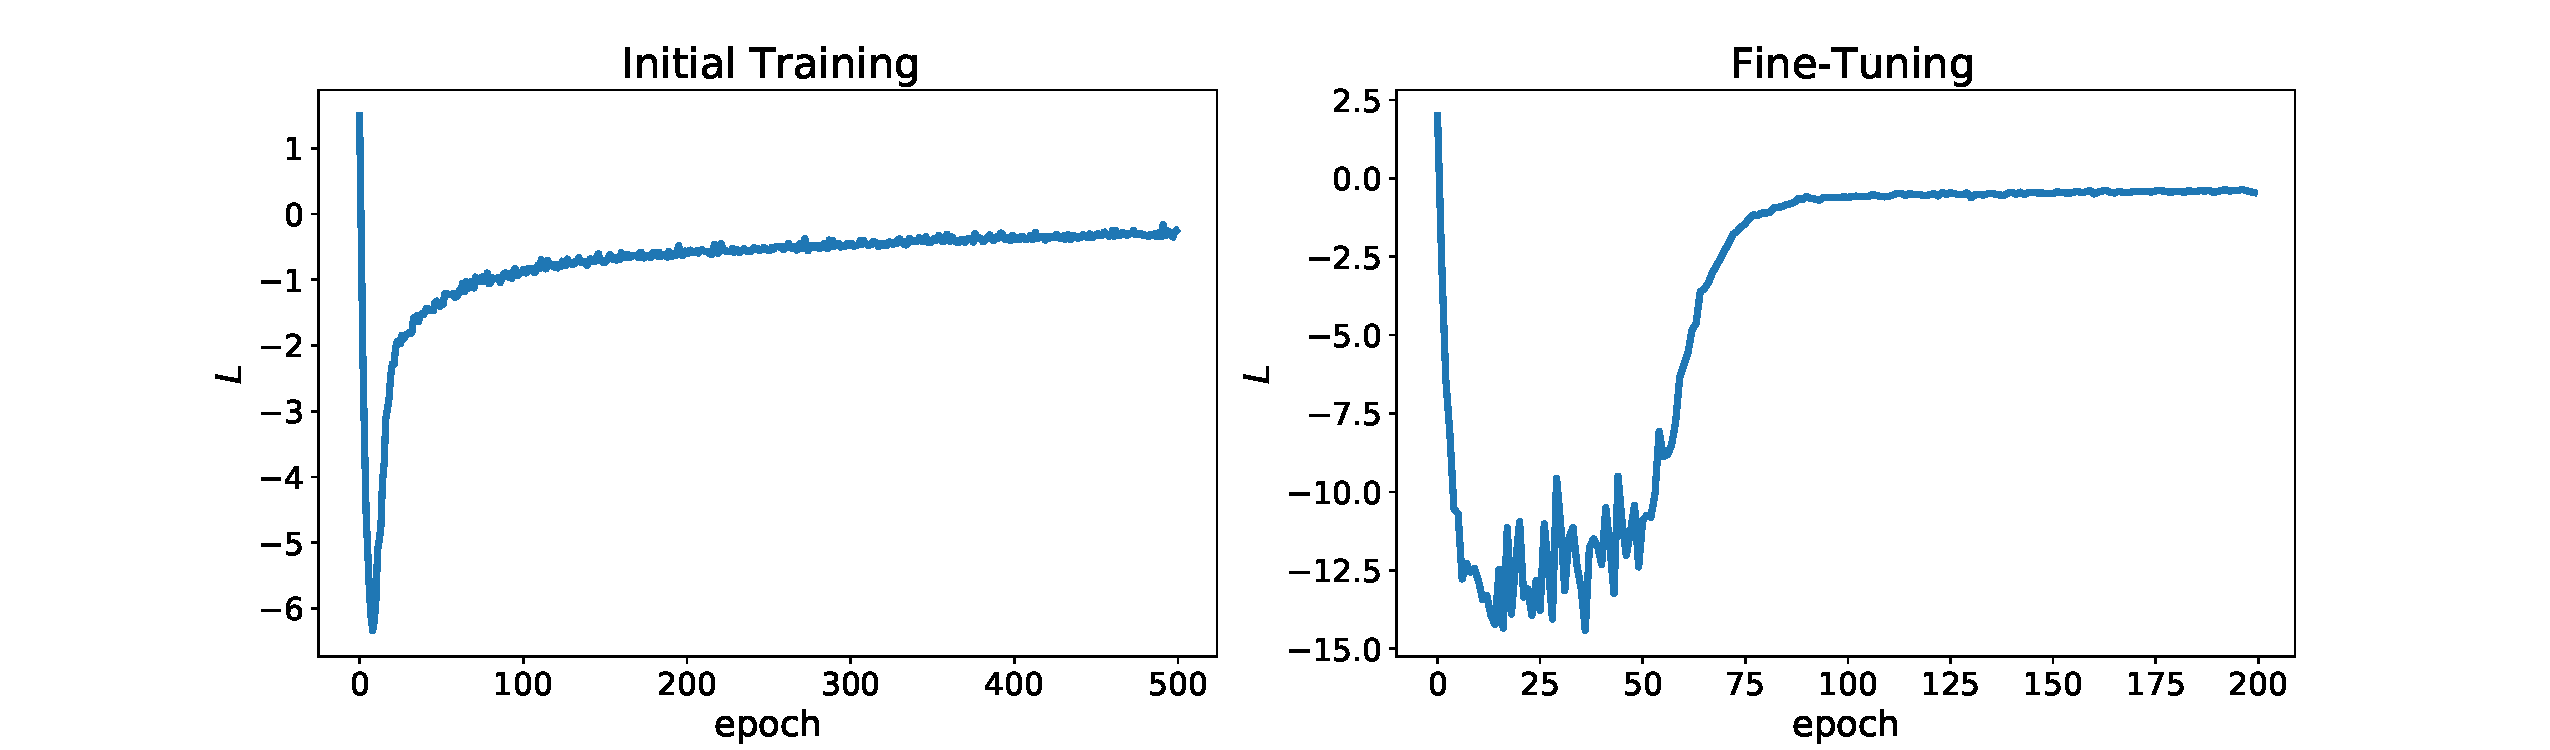
\includegraphics[width=1.2\textwidth]{figs/loss_main_evec_wgangp.pdf}}
    \caption{The loss functions of the critic of the WGAN-GP for the main eigenvector generation, respectively while performing the initial training and while fine-tuning}
    \label{fig:loss_main_evec_wgangp}
\end{figure}

Unlike for the eigenvalues, showing a generated sample of main eigenvector will not provide insights for assessing the quality of the generated sample. Therefore, instead the following was done: generate a sample main eigenvector $\hat{\mathbf{v}}_{63}$ and use equation \ref{rank_I_csm} to create a rank I CSM. It is important to note that the eigenvalue $\mathbf{\Lambda}_{63, 63}$ corresponding to the main eigenvector is by definition equal to one. Indeed, it is by definition the biggest eigenvalues and the eigenvalues were scaled such that all eigenvalues lie in $[0,1]$.  In Fig.~\ref{fig:beamforming_map_main_evec_wgangp} is plotted first the beamforming map resulting from performing beamforming with the Rank I CSM created from a sampled main eigenvector. In the second map of Fig.~\ref{fig:beamforming_map_main_evec_wgangp} is plotted the difference between a beamforming map computed with a generated main eigenvector and the beamforming map computed with a main eigenvector from the measurement dataset (i.e. map shown in Fig.~\ref{fig:measurement_sample_rank_I_beamforming}. It can observe that the difference of the two map is almost zero everywhere.

\begin{figure}
    \centering
    \begin{subfigure}{0.45\textwidth}
        \centering
        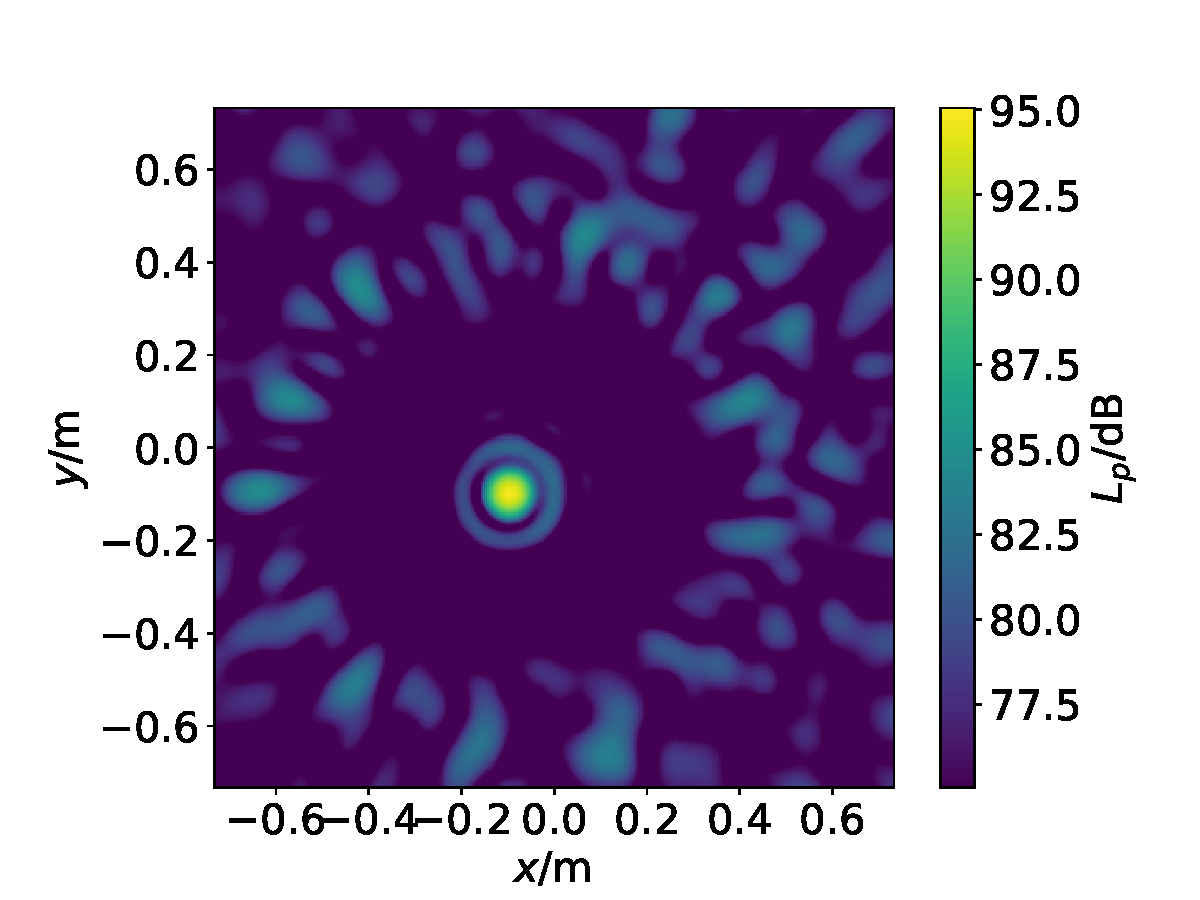
\includegraphics[width=1.3\textwidth]{figs/beamforming_map_main_evec_wgangp_generated.pdf}
        \caption{Generated Rank I CSM}
        \label{fig:beamforming_map_main_evec_wgangp_generated}
    \end{subfigure}
    \hfill
    \begin{subfigure}{0.45\textwidth}
        \centering
        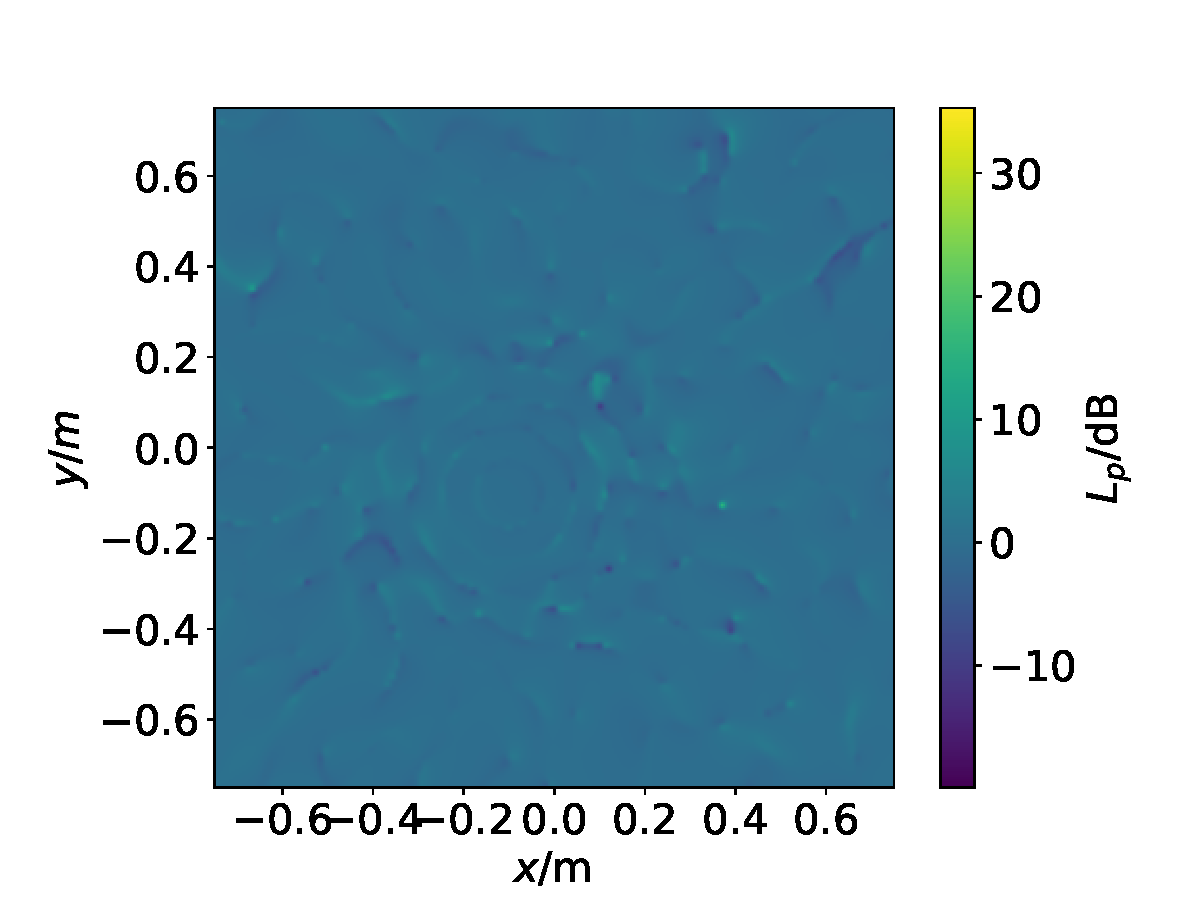
\includegraphics[width=1.3\textwidth]{figs/beamforming_map_main_evec_wgangp_difference.pdf}
        \caption{Difference}
        \label{fig:beamforming_map_main_evec_wgangp_difference}
    \end{subfigure}
    \caption{The first beamforming map has been perfomed with a Rank I CSM computed with a generated main eigenvector. The second map shows the difference between the beamforming map obtained with Rank I CSM computed respectively with a generated main eigenvector and a main eigenvector from the dataset.}
    \label{fig:beamforming_map_main_evec_wgangp}
\end{figure}


Moreover, 10000 sample main eigenvector were generated using the WGAN-GP and the one with the lowest critic score was used to create a beamforming map and plotted in Fig.~\ref{fig:outliers_main_evec}. It can be observed that the obtained map is almost identical to the one displayed in Fig.~\ref{fig:beamforming_map_main_evec_wgangp_generated}  

\begin{figure}
    \centering
    \makebox[\textwidth][c]{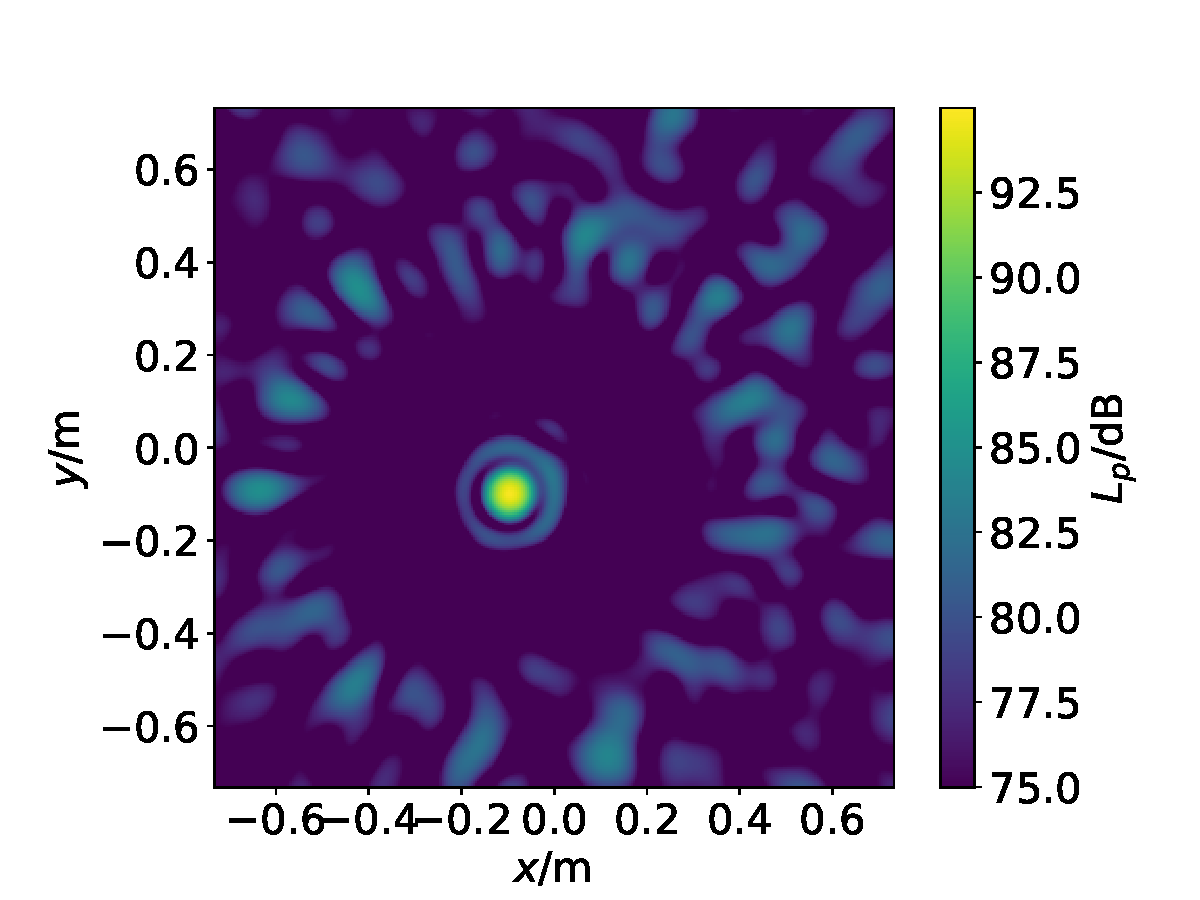
\includegraphics[width=0.6\textwidth]{figs/outliers_main_evec.pdf}}
    \caption{Beamforming map resulting from a rank I CSM, computed from a generated main eigenvector with the lowest critic score out of 10000 generated main eigenvector.}
    \label{fig:outliers_main_evec}    
\end{figure}

\subsection{Data Augmentation}

Three different beamforming map are displayed in Fig.~\ref{fig:data_augmentation_evecs}. Fig.~\ref{fig:data_augmentation_evecs_synthetic}, Fig.~\ref{fig:data_augmentation_evecs_measurement} and Fig.~\ref{fig:data_augmentation_evecs_augmented_csm} show respectively the beamforming map obtained when using a synthetic CSM, a measured CSM and a CSM augmented with generated eigenvalues. It can be observed that the map issued from an CSM augmented with a generated main eigenvector, displays thicker lobes than on the map issued from synthetic CSM, while not being fully identical to the map from issued from a measured CSM.



\begin{figure}
    \centering
    \begin{subfigure}{0.45\textwidth}
        \centering
        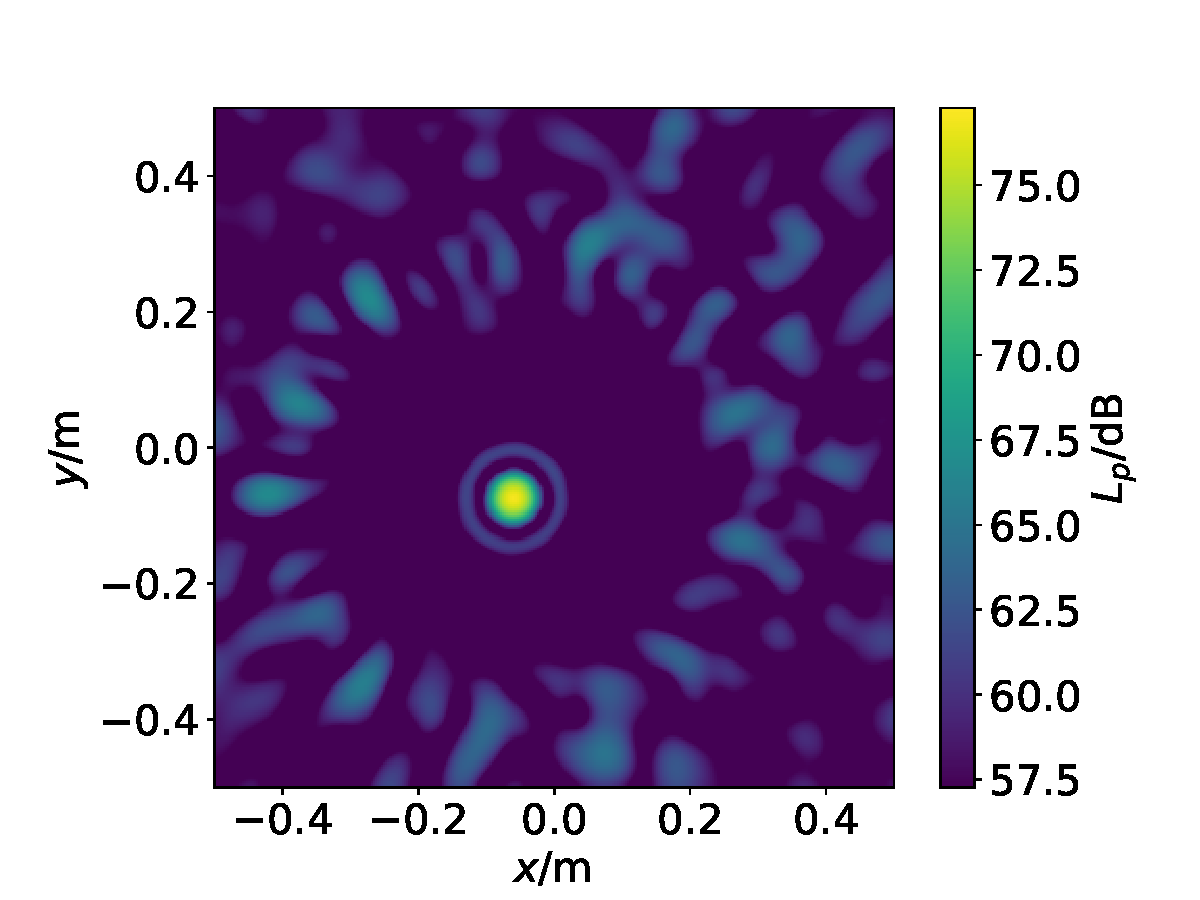
\includegraphics[width=1.3\textwidth]{figs/datasets_beamforming_example_synthetic.pdf}
        \caption{CSM from synthetic dataset}
        \label{fig:data_augmentation_evecs_synthetic}
    \end{subfigure}
    \hfill
    \begin{subfigure}{0.45\textwidth}
        \centering
        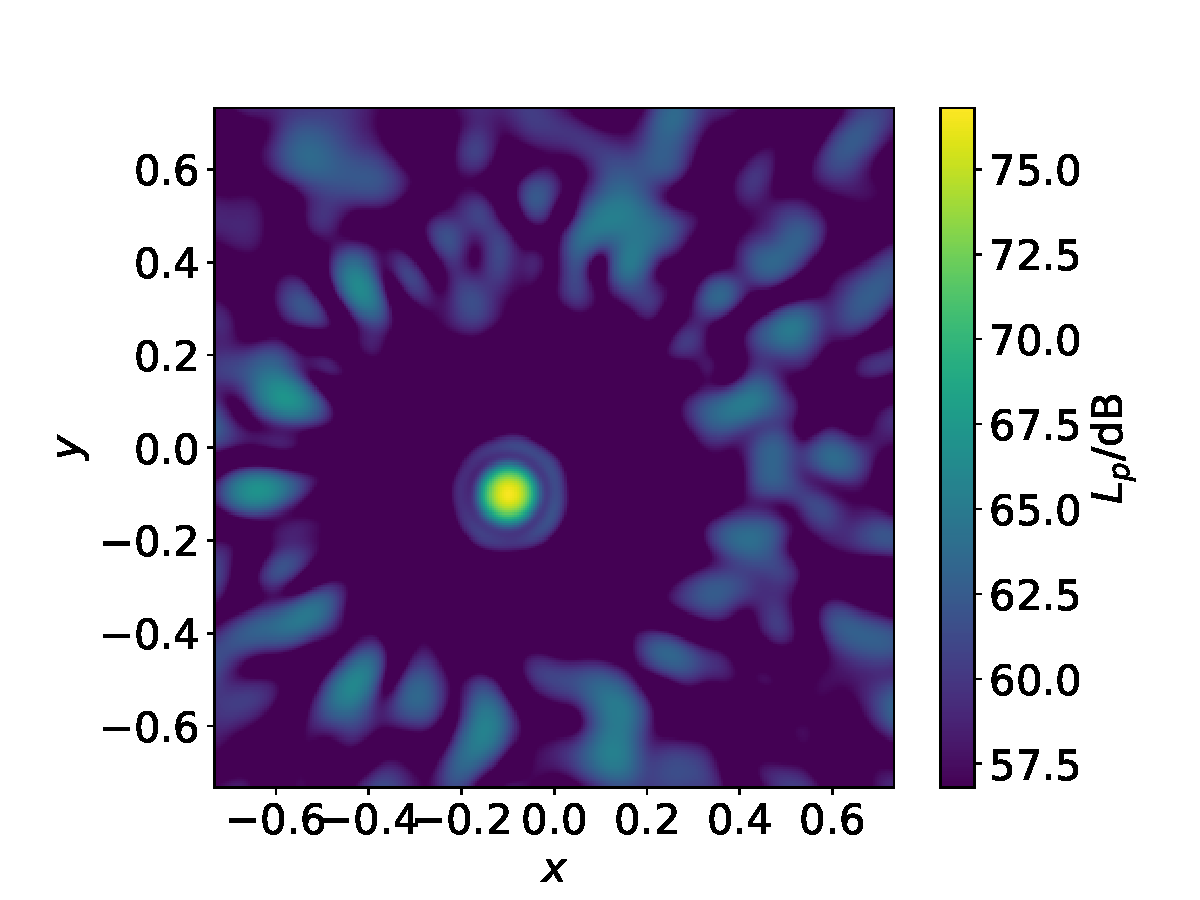
\includegraphics[width=1.3\textwidth]{figs/datasets_beamforming_example_measurement.pdf}
        \caption{CSM from measurement dataset}
        \label{fig:data_augmentation_evecs_measurement}
    \end{subfigure}
    \hfill
    \begin{subfigure}{0.45\textwidth}
        \centering
        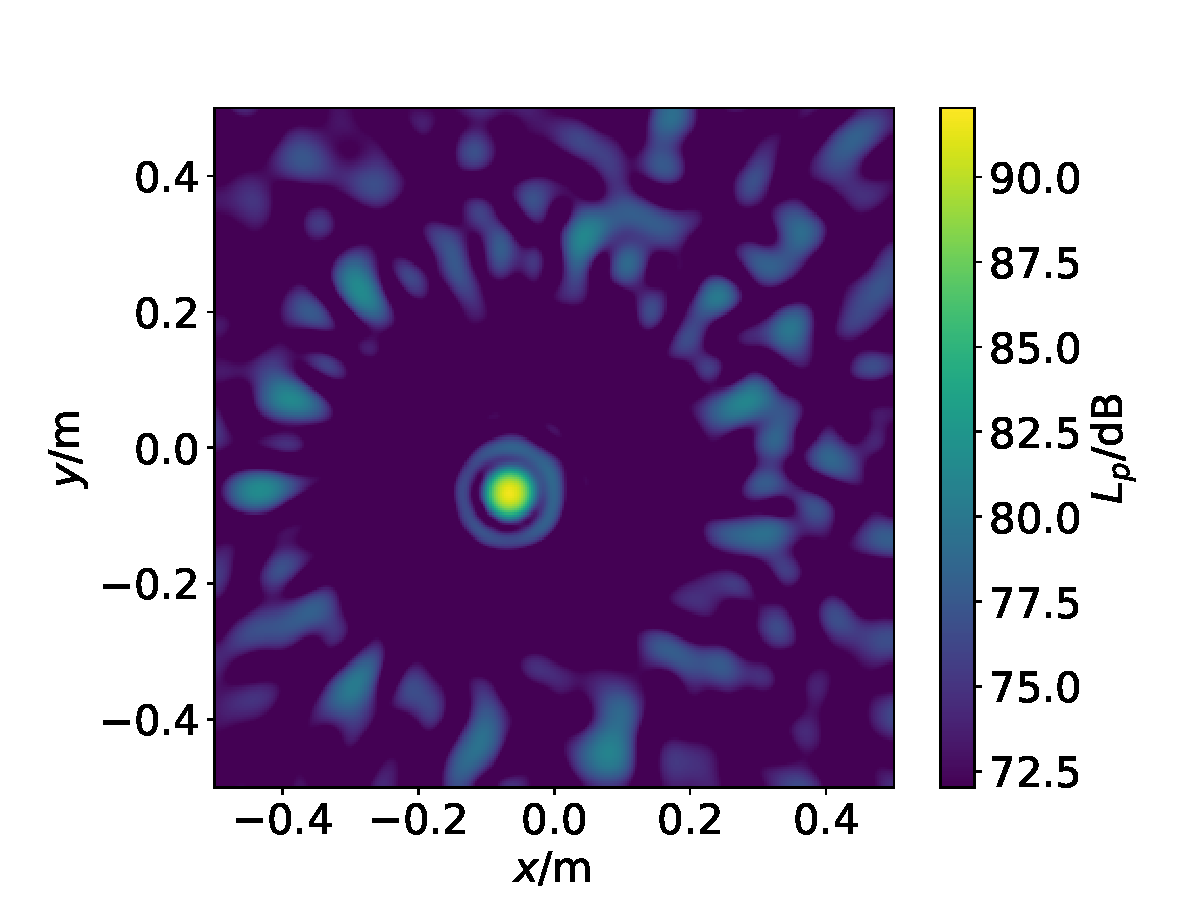
\includegraphics[width=1.3\textwidth]{figs/data_augmentation_evecs_augmented_csm.pdf}
        \caption{CSM Augmented From Main Eigenvector} 
        \label{fig:data_augmentation_evecs_augmented_csm}
    \end{subfigure}
            
    \caption{Three beamforming maps obtained from synthetic CSM, measured CSM and CSM augmented with generated main eigenvector}
    \label{fig:data_augmentation_evecs}
\end{figure}

\chapter{Discussions}

\section{Generating Eigenvalues}

\subsection{Generating Eigenvalues from their Scaled Values}

It was observed in the first plot of Fig.~\ref{fig:samples_evals_wgangp} that the difference between real and generated samples was obvious, when their level values are displayed. This can be explained by the fact, that the WGAN-GP cannot capture very well small numerical variation. This lack of extreme precision is very visible in the eigenvalues close to zero. Indeed, micro-variations around zero lead to big variations in the level values. Since the level of the spectrum, is the way used to tell synthetic data from measured data, using a Generative approach producing eigenvalues with unrealistic levels spectrum is not conceivable. 

\subsection{Generating Eigenvalues from their Level Values}

It can be observed that learning the levels of the eigenvalues leads to a network that is able to generate sample levels of eigenvalues more realistic than when generating sample eigenvalues and then computing their levels. This is due to the fact that the logarithm re-weights the generated values here, so that small values become more important for the critic. It can be concluded than this second method is better suited for generating eigenvalues of CSM.

Moreover, it was observed that training the network first with synthetic data and then fine-tuning it with a single measurement allows to produce eigenvalues that are not simply a data copy of the measured eigenvalues. Indeed, while the eigenvalues of a single measurement do not have a large variation, the produced sample eigenvalues cover a larger range. Hence, it can be concluded that this approach allows to generate eigenvalues samples that are representative not only of a single measurement, but of multiple ones. Moreover, it is important to notice, that these differences observed in the levels between generated and real eigenvalues, occur for eigenvalues that are very close to zero. Hence, these differences are not visible between real and generated eigenvalues, once converted back from their levels values.


\subsection{Data Augmentation}

It was observed that when using the data augmentation scheme with eigenvalues, the obtained beamforming map were still very similar to the ones obtained with synthetic CSM. It can therefore be concluded that only replacing the synthetic eigenvalues with more realistic eigenvalues is not sufficient to create realistic CSM.

\section{Generating Eigenvectors}

\subsection{Generating the Main Eigenvector}

When observing the beamforming map computed from generated main eigenvector, it can be concluded that WGAN-GP is able to generate sample close to the original main eigenvector, without being 100\% similar. Indeed, on the beamforming map, the audio source can be easily located, and the difference of between two beamforming map is not zero everywhere.

Though it is to be noted that when plotting an outlier, i.e. the sample with the lowest critic score amongst 10000 samples, the resulting beamforming map remains close to a sample with a higher score. From this it can be concluded that the WGAN-GP cannot produce a great variety of sample, but it is important to note that it is representative of the data it was trained with.  

\subsection{Data Augmentation}

The method introduced for data augmentation with the main eigenvector has shown to produce more satisfying results than with the eigenvalues. It was observed that when using the augmented CSM for beamforming, the resulting CSM both showed reliable information regarding source information but were also closer to the measured CSM. Indeed, the lobes on the resulting beamforming map were thicker than on the beamforming maps computed with a synthetic CSM.

Moreover, it is important to note that  this technique is very efficient and does not require a lot of computational effort. Indeed, training the WGAN-GP to produce  the eigenvectors takes approximately two minutes to train, and once the network's weights are computed, sample main eigenvector can be obtained instantly.

\section{General}

The data generated is accurate. Indeed, when replacing real data by generated data, in the case of rank I beamforming or data augmentation for the eigenvalues, beamforming could be performed providing with sufficiently clear beamforming map. But unfortunately, the data that can be currently generated, is not sufficient to create fully realistic CSM. Indeed, the CSM that can be recreated with generated eigenvalues and main eigenvectors do not account fully for the noise information, since this information is contained in the eigenvectors with index $0$ to $62$. The problem of generating the 64 eigenvectors simultaneously is complex, since it is subject to the constraint that all vectors need to be orthogonal. 


\chapter{Conclusion}

As it has been shown, the WGAN-GP introduced for generating eigenvalues from their level approach is able to produce realistic samples, which is not true when generating directly the eigenvalues. Moreover, it was shown that training this WGAN-GP with synthetic data and fine-tuning it with a single measurement was sufficient to produce a variety of different realistic spectra, also representative of the spectra of different measurement, not used for training.  

Then, it is shown that a WGAN-GP approach is also suited to generate realistic strongest eigenvector. The beamforming map generated from Rank I CSM computed with generated strongest eigenvector showed accuratly the position of the sound source.

Moreover, the data augmentation method using generated main eigenvector allows to improve how realistic synthetic CSM are. It was shown that the beamforming map obtained from CSM augmented with this method displayed features of beamforming map obtained from measurement data.

In conclusion, it can be stated that this thesis lay important foundation for generating the CSM representation of microphone array data. It introduces new methods for learning matrix data, by using its eigendecomposition. It is shown that the eigedecomposition is a good representation of CSM to learn their distribution and hence generating them. The finding in this thesis are an important step toward solving the unavailability of real training data for source localization or characterization. Indeed, as shown in the literature survey, extensive researchs on this topic do not exist, which makes the contribution of this thesis especially relevant. 


\chapter{Future Works}

For the purpose of generating realistic CSM for training DL-based algorithm for source characterization, the methods introduced in this thesis would need to be extended to be able to generate CSM for different positions. More specifically, this would need to be done for the network to generate the main eigenvector. Indeed, the eigenvalue spectrum is not position dependent, hence no modification is needed to the current network for a later use in generating CSM for multiple positions.

More than simply training the eigenvectors for multiple positions, it should be investigated whether a Neural Network could be designed for generating eigenvectors also corresponding to source position not observed in the dataset. It is to be noted that a good starting point for this investigation would be to attempt to build a Neural Network to learn relationship between source position and the main eigenvector.

In is also to be noted that in order to generate realistic CSM, its is crucial to be able to model the weakest eigenvectors. i.e. the eigenvectors with index $0$ to $62$. Extending the approach to generate the strongest eigenvector to all eigenvectors, has been tried but without compelling results. An idea that could be tried is that instead of feeding real and generated eigenvectors to the critic, the corresponding beamforming map could be computed and fed to the critic. The architecture of the critic would then need to be converted from a perceptron architecture to a convolutional one. 


\cleardoublepage

%%%%%%%%%%%%%%%%%%%%%%%%%%%%%%%%%%%%%%%%%%%%%%%%%%%%%%%%%%%%%%%%%%%%%%%%%%%%%%%
%%%%% Appendices (optional)
%%%%%%%%%%%%%%%%%%%%%%%%%%%%%%%%%%%%%%%%%%%%%%%%%%%%%%%%%%%%%%%%%%%%%%%%%%%%%%%
\appendix
\fancyhead[LO]{\rightmark}
\fancyhead[RO]{\scshape\appendixname\ \thechapter}
\fancyhead[LE]{\scshape\appendixname\ \thechapter}
\fancyhead[RE]{\textsc{\leftmark}}


\chapter[Architectures of the Different Networks]{Architectures of the Generator and Critic Networks}

In this appendix are compiled the architectures of the critics and generators used in the different WGAN-GP designed for this thesis:

\begin{itemize}
    \item Tab.~\ref{tab:evals_generator_WGANGP_architecture} shows the architecture of the generator used in the WGAN-GP for generating the eigenvalues from their scaled values.
    \item Tab.~\ref{tab:evals_critic_WGANGP_architecture} shows the architecture of the critic used in the WGAN-GP for generating the eigenvalues from their scaled values.
    \item Tab.~\ref{tab:evals_dB_generator_WGANGP_architecture} shows the architecture of the generator used in the WGAN-GP for generating the eigenvalues from their levels.
    \item Tab.~\ref{tab:evals_dB_critic_WGANGP_architecture} shows the architecture of the critic used in the WGAN-GP for generating the eigenvalues from their levels.
    \item Tab.~\ref{tab:main_evec_generator_WGANGP_architecture} shows the architecture of the generator used in the WGAN-GP for generating the main eigenvector.
    \item Tab.~\ref{tab:main_evec_critic_WGANGP_architecture} shows the architecture of the critic used in the WGAN-GP for generating the main eigenvector.
\end{itemize}


\begin{table}[]
  \centering
  \begin{tabular}{c c c}
      \hline
      \textbf{Layer} & \textbf{Output Shape} & \textbf{Number of Parameters} \\ \hline
      InputLayer            & 128           & 0                 \\ 
      Dense                 & 256           & 32768             \\ 
      LeakyReLU             & 256           & 0                 \\ 
      BatchNormalization    & 256           & 1024              \\ 
      Dense                 & 512           & 131584            \\ 
      LeakyReLU             & 512           & 0                 \\ 
      Dense                 & 1024          & 525312            \\ 
      LeakyReLU             & 1024          & 0                 \\ 
      Dense                 & 64            & 65600             \\ 
      \end{tabular}
  \caption{Architecture of the generator used in the WGAN-GP to generate eigenvalues. Total parameters: 756,288, Trainable parameters: 755,776, Non-trainable parameters: 512}
  \label{tab:evals_generator_WGANGP_architecture}
\end{table}

\begin{table}[]
  \centering
  \begin{tabular}{c c c}
      \hline
      \textbf{Layer} & \textbf{Output Shape} & \textbf{Number of Parameters} \\ \hline
      InputLayer            & 64            & 0                 \\
      Dense                 & 512           & 33280             \\
      LeakyReLU             & 512           & 0                 \\
      Dense                 & 256           & 131328            \\
      LeakyReLU             & 256           & 0                 \\
      Dense                 & 1             & 257               \\
  \end{tabular}
  \caption{Architecture of the critic used in the WGAN-GP to generate eigenvalues. Total parameters: 164,865, Trainable parameters: 164,865, Non-trainable parameters: 0}
  \label{tab:evals_critic_WGANGP_architecture}
\end{table}

\begin{table}[]
  \centering
  \begin{tabular}{c c c}
      \hline
      \textbf{Layer} & \textbf{Output Shape} & \textbf{Number of Parameters} \\ \hline
      InputLayer            & 128           & 0                 \\
      Dense                 & 256           & 32768             \\
      LeakyReLU             & 256           & 0                 \\
      BatchNormalization    & 256           & 1024              \\
      Dense                 & 512           & 131584            \\
      LeakyReLU             & 512           & 0                 \\
      Dense                 & 1024          & 525312            \\
      LeakyReLU             & 1024          & 0                 \\
      Dense                 & 64            & 65600             \\
      ReLU                  & 64            & 0                 \\
      Multiply              & 64            & 0                 \\
  \end{tabular}
  \caption{Architecture of the generator used in the WGAN-GP to generate eigenvalues from their level values. Total parameters: 756,288, Trainable parameters: 755,776, Non-trainable parameters: 512}
  \label{tab:evals_dB_generator_WGANGP_architecture}
\end{table}

\begin{table}[]
  \centering
  \begin{tabular}{c c c}
      \hline
      \textbf{Layer} & \textbf{Output Shape} & \textbf{Number of Parameters} \\ \hline
      InputLayer            & 64            & 0                 \\
      Multiply              & 64            & 0                 \\
      Dense                 & 512           & 33280             \\
      LeakyReLU             & 512           & 0                 \\
      Dense                 & 256           & 131328            \\
      LeakyReLU             & 256           & 0                 \\
      Dense                 & 1             & 257               \\
  \end{tabular}
  \caption{Architecture of the critic used in the WGAN-GP to generate eigenvalues from their level values. Total parameters: 164,865, Trainable parameters: 164,865, Non-trainable parameters: 0}
  \label{tab:evals_dB_critic_WGANGP_architecture}
\end{table}

\begin{table}[]
  \centering
  \begin{tabular}{c c c}
      \hline
      \textbf{Layer} & \textbf{Output Shape} & \textbf{Number of Parameters} \\ \hline
      InputLayer            & 128           & 0                 \\
      Dense                 & 256           & 32768             \\
      LeakyReLU             & 256           & 0                 \\
      BatchNormalization    & 256           & 1024              \\
      Dense                 & 512           & 131584            \\
      LeakyReLU             & 512           & 0                 \\
      Dense                 & 1024          & 525312            \\
      LeakyReLU             & 1024          & 0                 \\
      Dense                 & 128           & 131200            \\
      Reshape               & (1, 64, 2)    & 0                 \\
  \end{tabular}
  \caption{Architecture of the generator used in the WGAN-GP to generate the main eigenvector. Total parameters: 821,888, Trainable parameters: 821,376, Non-trainable parameters: 512}
  \label{tab:main_evec_generator_WGANGP_architecture}
\end{table}

\begin{table}[]
  \centering
  \begin{tabular}{c c c}
      \hline
      \textbf{Layer} & \textbf{Output Shape} & \textbf{Number of Parameters} \\ \hline
      InputLayer            & (1, 64, 2)    & 0                 \\
      Flatten               & 128           & 0                 \\
      Dense                 & 512           & 66048             \\
      LeakyReLU             & 512           & 0                 \\
      Dense                 & 256           & 131328            \\
      LeakyReLU             & 256           & 0                 \\
      Dense                 & 1             & 257               \\
  \end{tabular}
  \caption{Architecture of the critic used in the WGAN-GP to generate the main eigenvector. Total parameters: 197,633, Trainable parameters: 197,633, Non-trainable parameters: 0}
  \label{tab:main_evec_critic_WGANGP_architecture}
\end{table}


\cleardoublepage

%%%%%%%%%%%%%%%%%%%%%%%%%%%%%%%%%%%%%%%%%%%%%%%%%%%%%%%%%%%%%%%%%%%%%%%%%%%%%%%
%%%%% Bibliography, List of Figures, List of Tables
%%%%%%%%%%%%%%%%%%%%%%%%%%%%%%%%%%%%%%%%%%%%%%%%%%%%%%%%%%%%%%%%%%%%%%%%%%%%%%%
\fancyhead[LO]{\scshape\bibname}
\fancyhead[RO]{}
\fancyhead[LE]{}
\fancyhead[RE]{\scshape\bibname}

% Bibliography
\bibliographystyle{IEEEtran} % bibliography style in order of first citation
\phantomsection\addcontentsline{toc}{chapter}{\numberline{}\bibname}
\bibliography{./resources/IEEEabrv,./bibliography}

\cleardoublepage

% List of figures (optional)
\fancyhead[LO]{\scshape \listfigurename}
\fancyhead[RO]{}
\fancyhead[LE]{}
\fancyhead[RE]{\scshape \listfigurename}
\phantomsection\addcontentsline{toc}{chapter}{\numberline{}\listfigurename}
\listoffigures

\cleardoublepage

% List of tables (optional)
\fancyhead[LO]{\scshape \listtablename}
\fancyhead[RO]{}
\fancyhead[LE]{}
\fancyhead[RE]{\scshape \listtablename}
\phantomsection\addcontentsline{toc}{chapter}{\numberline{}\listtablename}
\listoftables

%%%%%%%%%%%%%%%%%%%%%%%%%%%%%%%%%%%%%%%%%%%%%%%%%%%%%%%%%%%%%%%%%%%%%%%%%%%%%%%
%%%%% Declaration of Orginiality
%%%%%%%%%%%%%%%%%%%%%%%%%%%%%%%%%%%%%%%%%%%%%%%%%%%%%%%%%%%%%%%%%%%%%%%%%%%%%%%
\cleardoublepage
\fancyhead[LO]{}
\fancyhead[RO]{}
\fancyhead[LE]{}
\fancyhead[RE]{}



\includepdf[pages=-]{decl_originality.pdf}



\end{document}

%%% Local Variables:
%%% mode: latex
%%% TeX-master: t
%%% End:
